\section{CFD analýza konstrukčních úprav} \label{sec:konstrukcni-upravy}    
    \subsection{Studie citlivosti výpočetní sítě}
        Nutným předpokladem pro věrohodnost výpočtů je jejich dostatečná přesnost. Ta může být ovlivněna například vhodností použitého fyzikálního modelu, numerického schématu, ale také i kvalitou a jemností výpočetní sítě. Pro zahájení CFD testování konstruknčních úprav DRTA sondy bylo tak třeba se jako první zaměřit na vliv výpočetní sítě na výsledky výpočtů. Bylo testováno celkem sedm různých sítí s odlišně velikými elementy. Postup jejich tvorby odpovídá Kapitole \ref{sec:vypocetni-sit}, diverzity bylo dosaženo prostřednictvím změn parametrů povrchové sítě. Ty jsou společně s celkovými počty buněk uvedeny v Tabulce \ref{tab:citlivost-site}. Ostatní parametry sítě byly zachovány. Analýza byla provedena na výchozím modelu sondy s využitím roviny symetrie, viz Kapitola \ref{sec:sonda-bez-stineni-B}.

        \begin{table}[ht!]
            \centering
            \caption{Parametry síťování pro citlivostní analýzu sítě.}
            \resizebox{\textwidth}{!}{%
            \begin{tabular}{l|l|l|l|l|l|l|l}
                                                    & Síť 1  & Síť 2   & Síť 3   & Síť 4   & Síť 5   & Síť 6   & Síť 7   \\ \hline
            Minimální velikost elementů $\unit{mm}$ & 0.5    & 0.4     & 0.3     & 0.2     & 0.1     & 0.05    & 0.005   \\ \hline
            Maximální velikost elementů $\unit{mm}$ & 15     & 15      & 15      & 15      & 15      & 10      & 5       \\ \hline
            Výsledný počet buněk sítě $\unit{1}$    & 89 968 & 131 245 & 212 916 & 296 188 & 457 783 & 472 442 & 542 825
            \end{tabular}%
            }
            \label{tab:citlivost-site}
            \end{table}

        Vzhledem k cíli výpočtů byly jako sledované parametry zvoleny restituční faktory teplotních čidel. Jejich průběh v závislosti na použité síti je uveden na Obrázku \ref{fig:citlivost-site}. Zde je patrné, že u sítí $1 \div 4$ docházelo k výraznému nárůstu hodnot restitučních faktorů, zatímco u sítí $5 \div 7$ se hodnoty prakticky neměnily – bylo je tedy možné označit za vhodné kandidáty. Pro další výpočty byla zvolena síť $5$, nejhrubší z přijatelných sítí.

        \begin{figure}[ht!]
            \centering
            \includegraphics*[width=\textwidth]{400_SIMULACE_KONSTRUKCNICH_UPRAV/Grafy/citlivost_site.eps}
            \caption{Závislost restitučních faktorů sondy bez stínění čidla B na jemnosti výpočetní sítě.}
            \label{fig:citlivost-site}
        \end{figure}
    \newpage
    \subsection{Sonda bez stínění čidla B} \label{sec:sonda-bez-stineni-B}
        Analýzu konstrukčních úprav zahájilo zkoumání výchozí (a zároveň nejjednodušší) varianty sondy – s původními rozměry stínění čidla A a bez jakéhokoli odstínění čidla B. Cílem bylo určit problematická místa, která bude vhodné zkoumat jako první. Použitý model je znázorněn na Obrázku \ref{fig:sonda-bez-stineni-B}, konkrétní rozměry jsou uvedeny v Příloze \ref{fig:sonda-bez-stineni-B-vykres}. 

        \begin{figure}[ht!]
            \centering
            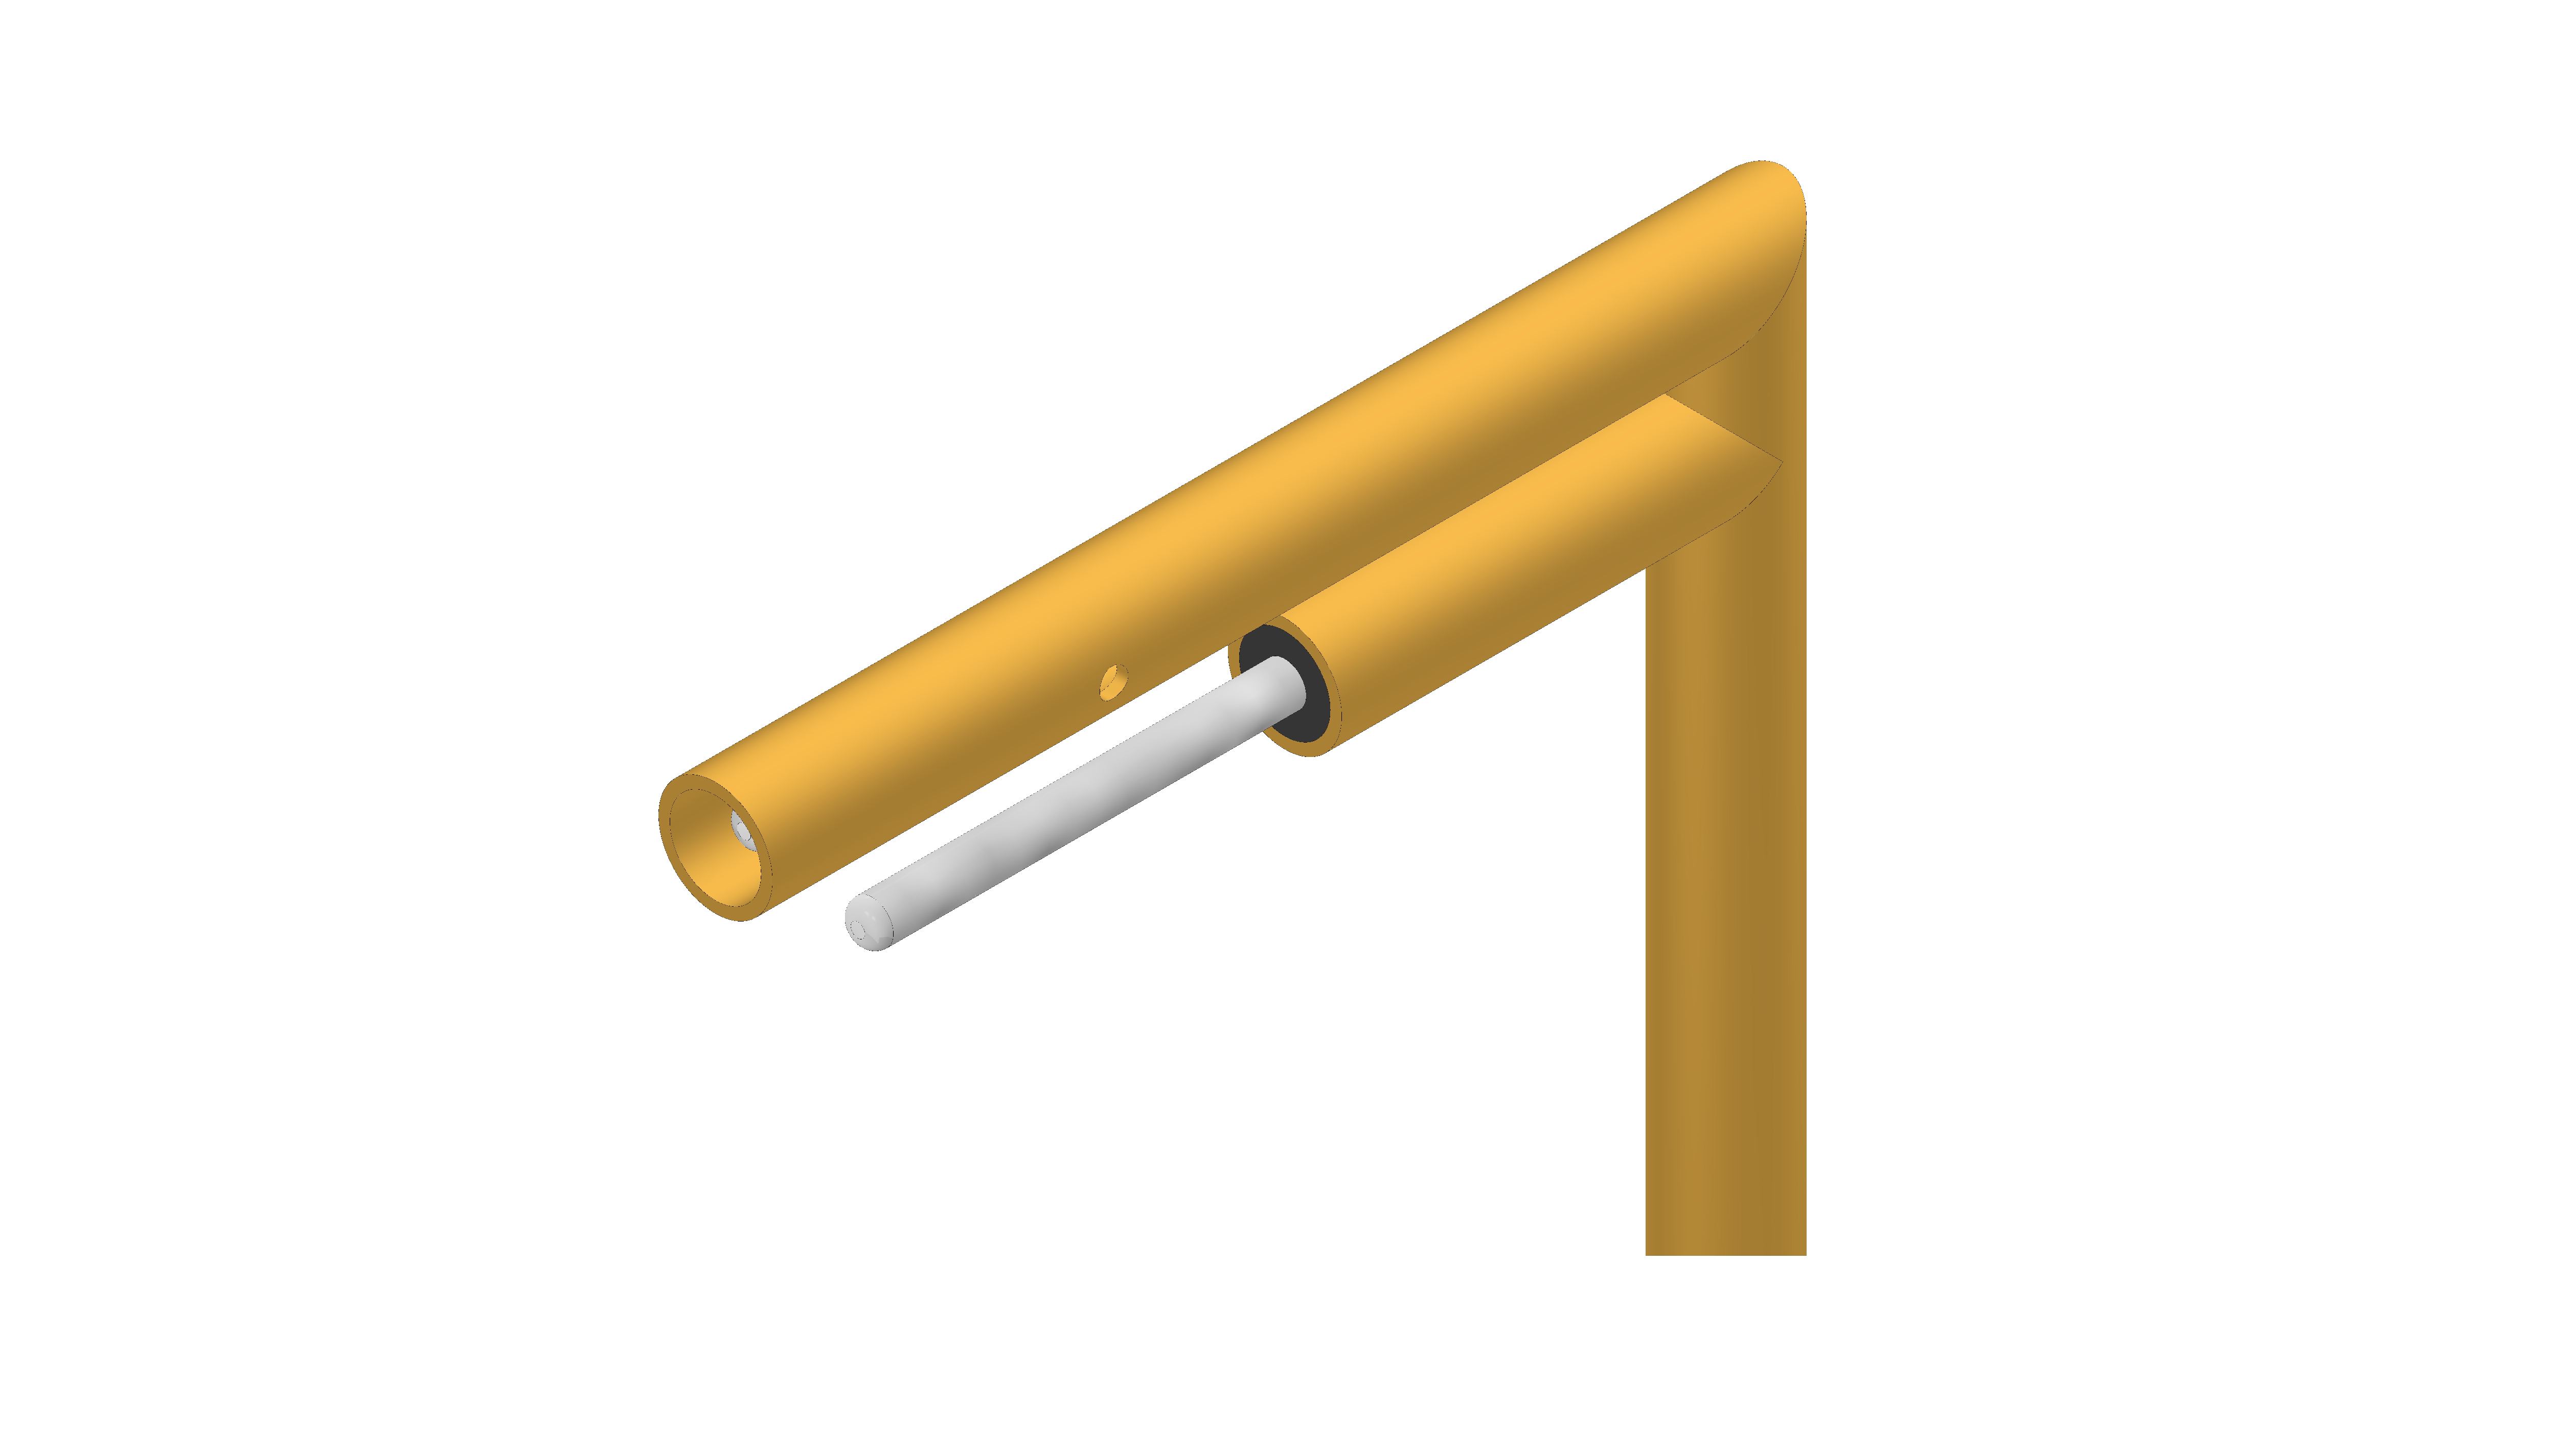
\includegraphics[width=\textwidth]{400_SIMULACE_KONSTRUKCNICH_UPRAV/Vykresy_rendery/Sonda_bez_stineni_B.png}
            \caption{Sonda bez stínění čidla B.}
            \label{fig:sonda-bez-stineni-B}
        \end{figure}
        
        Zkoumáno bylo chování restitučních faktorů při různých rychlostech nabíhajícího proudu v rozmezí $100 \div 325 \unit{\frac{m}{s}}$ s krokem $25 \Unit{\frac{m}{s}}$ a při vychýlení sondy ve dvou rovinách – v rovině symetrie $XY$ (natočení značeno jako $\varphi _Z$) a poté kolmo na rovinu symetrie (rovina $XZ$, značeno $\varphi _Y$), v obou případech s krokem $2.5^o$ v rozmezí $\pm 15^o$.
        
        \newpage
        \subsubsection{Chování při různých rychlostech proudění}
            Výsledky výpočtu jsou znázorněny v Obrázku \ref{fig:sonda-bez-stineni-rychlosti}. Z průběhu restitučního faktoru čidla B lze usuzovat, že docházelo k výraznějšímu ovlivnění proudění v jeho blízkosti vlivem stínění čidla A. To je patrné i z Obrázku \ref{fig:sonda-bez-stineni-vizualizace}. 
            
            \begin{figure}[ht!]
                \centering
                \includegraphics*[width=\textwidth]{400_SIMULACE_KONSTRUKCNICH_UPRAV/Grafy/01_rychlosti.eps}
                \caption{Závislost restitučních faktorů sondy bez stínění čidla B na rychlosti proudění.}
                \label{fig:sonda-bez-stineni-rychlosti}
            \end{figure}

            \begin{figure}[ht!]
                \centering
                \begin{subfigure}{0.45\textwidth}
                    \centering
                    \captionsetup{width=.9\linewidth}
                    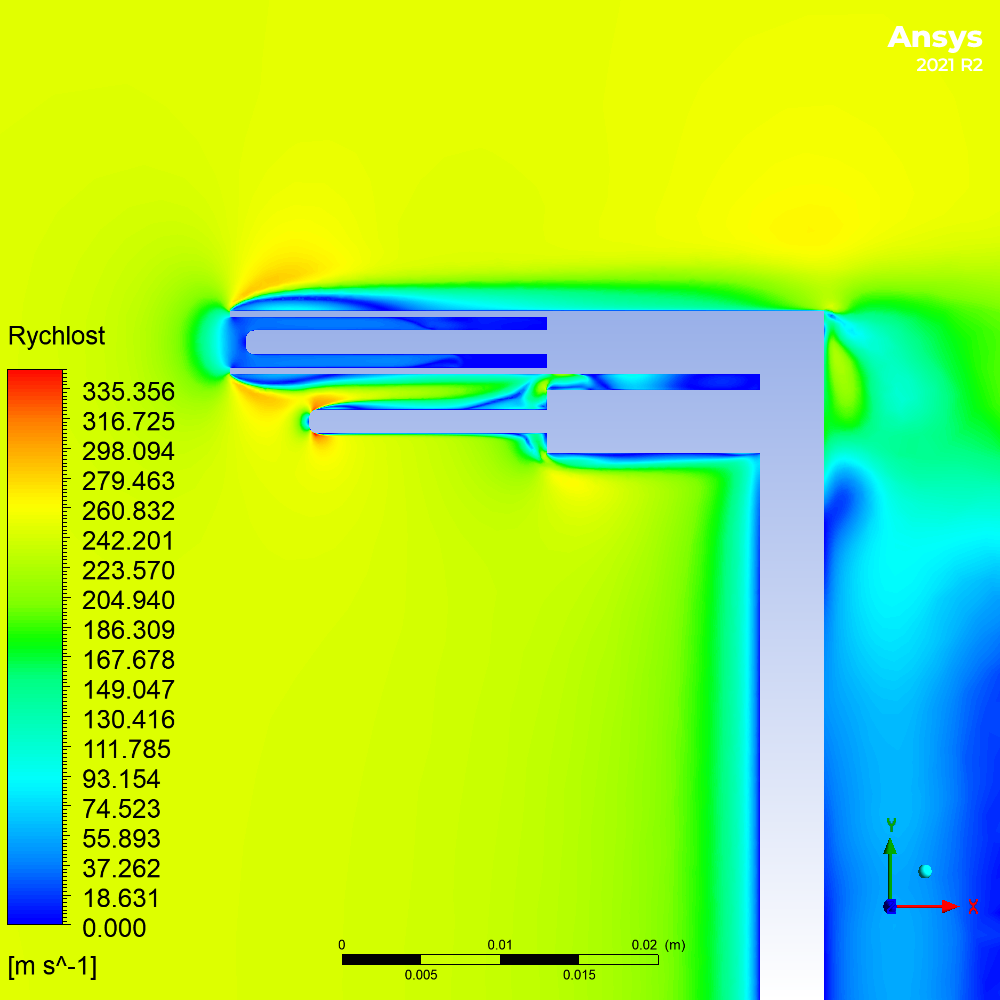
\includegraphics[width=\textwidth]{400_SIMULACE_KONSTRUKCNICH_UPRAV/Vizualizace/sonda_bez_stineni_vizualizace_rychlost.png}
                    \caption{Rychlostní pole.}
                \end{subfigure}
                \begin{subfigure}{0.45\textwidth}
                    \centering
                    \captionsetup{width=.9\linewidth}
                    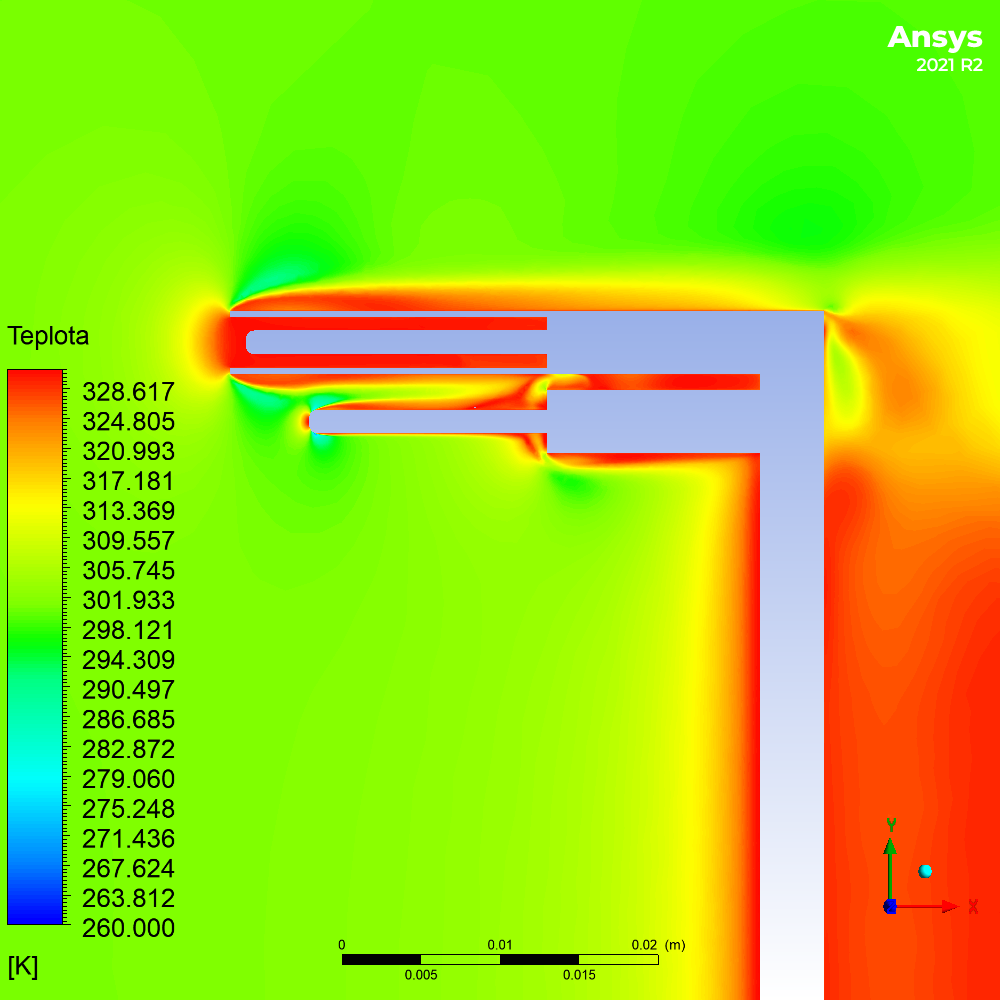
\includegraphics[width=\textwidth]{400_SIMULACE_KONSTRUKCNICH_UPRAV/Vizualizace/sonda_bez_stineni_vizualizace_teplota.png}
                    \caption{Teplotní pole.}
                \end{subfigure}
                \caption{Vizualizace vypočtených dat pro sondu bez stínění čidla B v rovině symetrie pro rychlost proudění $250 \Unit{\frac{m}{s}}$.}
                \label{fig:sonda-bez-stineni-vizualizace}
            \end{figure}


        \newpage
        \subsubsection{Směrová citlivost v rovině symetrie}
            Při natáčení sondy směrem dolů (tedy v záporném smyslu otáčení, kdy proud směřuje na vršek sondy) docházelo k zastínění čidla B, které se tak nacházelo částečně v\,úplavu trubice stínící čidlo A. To způsobilo výraznou změnu jeho restitučního faktoru, jak je patrné z Obrázku \ref{fig:sonda-bez-stineni-rovina-symetrie} – relativní odchylka od hodnoty nevychýlené sondy byla pro natočení $-15^o$ rovna $7.4 \Unit{\%}$. Při natočení sondy opačným směrem nedocházelo k\,výrazným výchylkám restitučních faktorů, zde relativní odchylka nepřekročila $0.2 \Unit{\%}$.
            
            \begin{figure}[ht!]
                \centering
                \includegraphics*[width=\textwidth]{400_SIMULACE_KONSTRUKCNICH_UPRAV/Grafy/01_rovina_symetrie}
                \caption{Závislost restitučních faktorů sondy bez stínění čidla B na natočení sondy v rovině symetrie.}
                \label{fig:sonda-bez-stineni-rovina-symetrie}
            \end{figure}
        \subsubsection{Směrová citlivost kolmo na rovinu symetrie}
            Vychýlení sondy kolmo na rovinu symetrie neukázalo žádné vážné problémy (viz Obrázek \ref{fig:sonda-bez-stineni-kolma-rovina}). Nejvyšší relativní odchylka restitučních faktorů nepřekročila $1.4 \Unit{\%}$ u\,čidla\,A a $1.8 \Unit{\%}$ u čidla B.
            
             \begin{figure}[ht!]
                \centering
                \includegraphics*[width=\textwidth]{400_SIMULACE_KONSTRUKCNICH_UPRAV/Grafy/01_kolma_rovina}
                \caption{Závislost restitučních faktorů sondy bez stínění čidla B na natočení kolmo na rovinu symetrie.}
                \label{fig:sonda-bez-stineni-kolma-rovina}
            \end{figure}

        \subsubsection{Zhodnocení}
            Problematickým místem první verze sondy se ukázalo čidlo B, které bylo ovlivňováno stíněním čidla A jak při změnách rychlosti proudění, tak při změnách natočení sondy. Prvním návrhem konstrukční úpravy tak bylo jeho odstínění.
    \newpage
    \subsection{Sonda se stíněním čidla B} \label{sec:sonda-se-stinenim-B}
        Odstínění čidla B bylo zajištěno pomocí trubice $5.8 \times 0.4 \Unit{mm}$ uchycené ke stínění čidla A, viz Obrázek \ref{fig:sonda-se-stinenim-B}. Detailní geometrie spolu s použitými rozměry modelu jsou uvedeny v Příloze \ref{fig:sonda-se-stinenim-B-vykres}. 
        
        \begin{figure}[ht!]
            \centering
            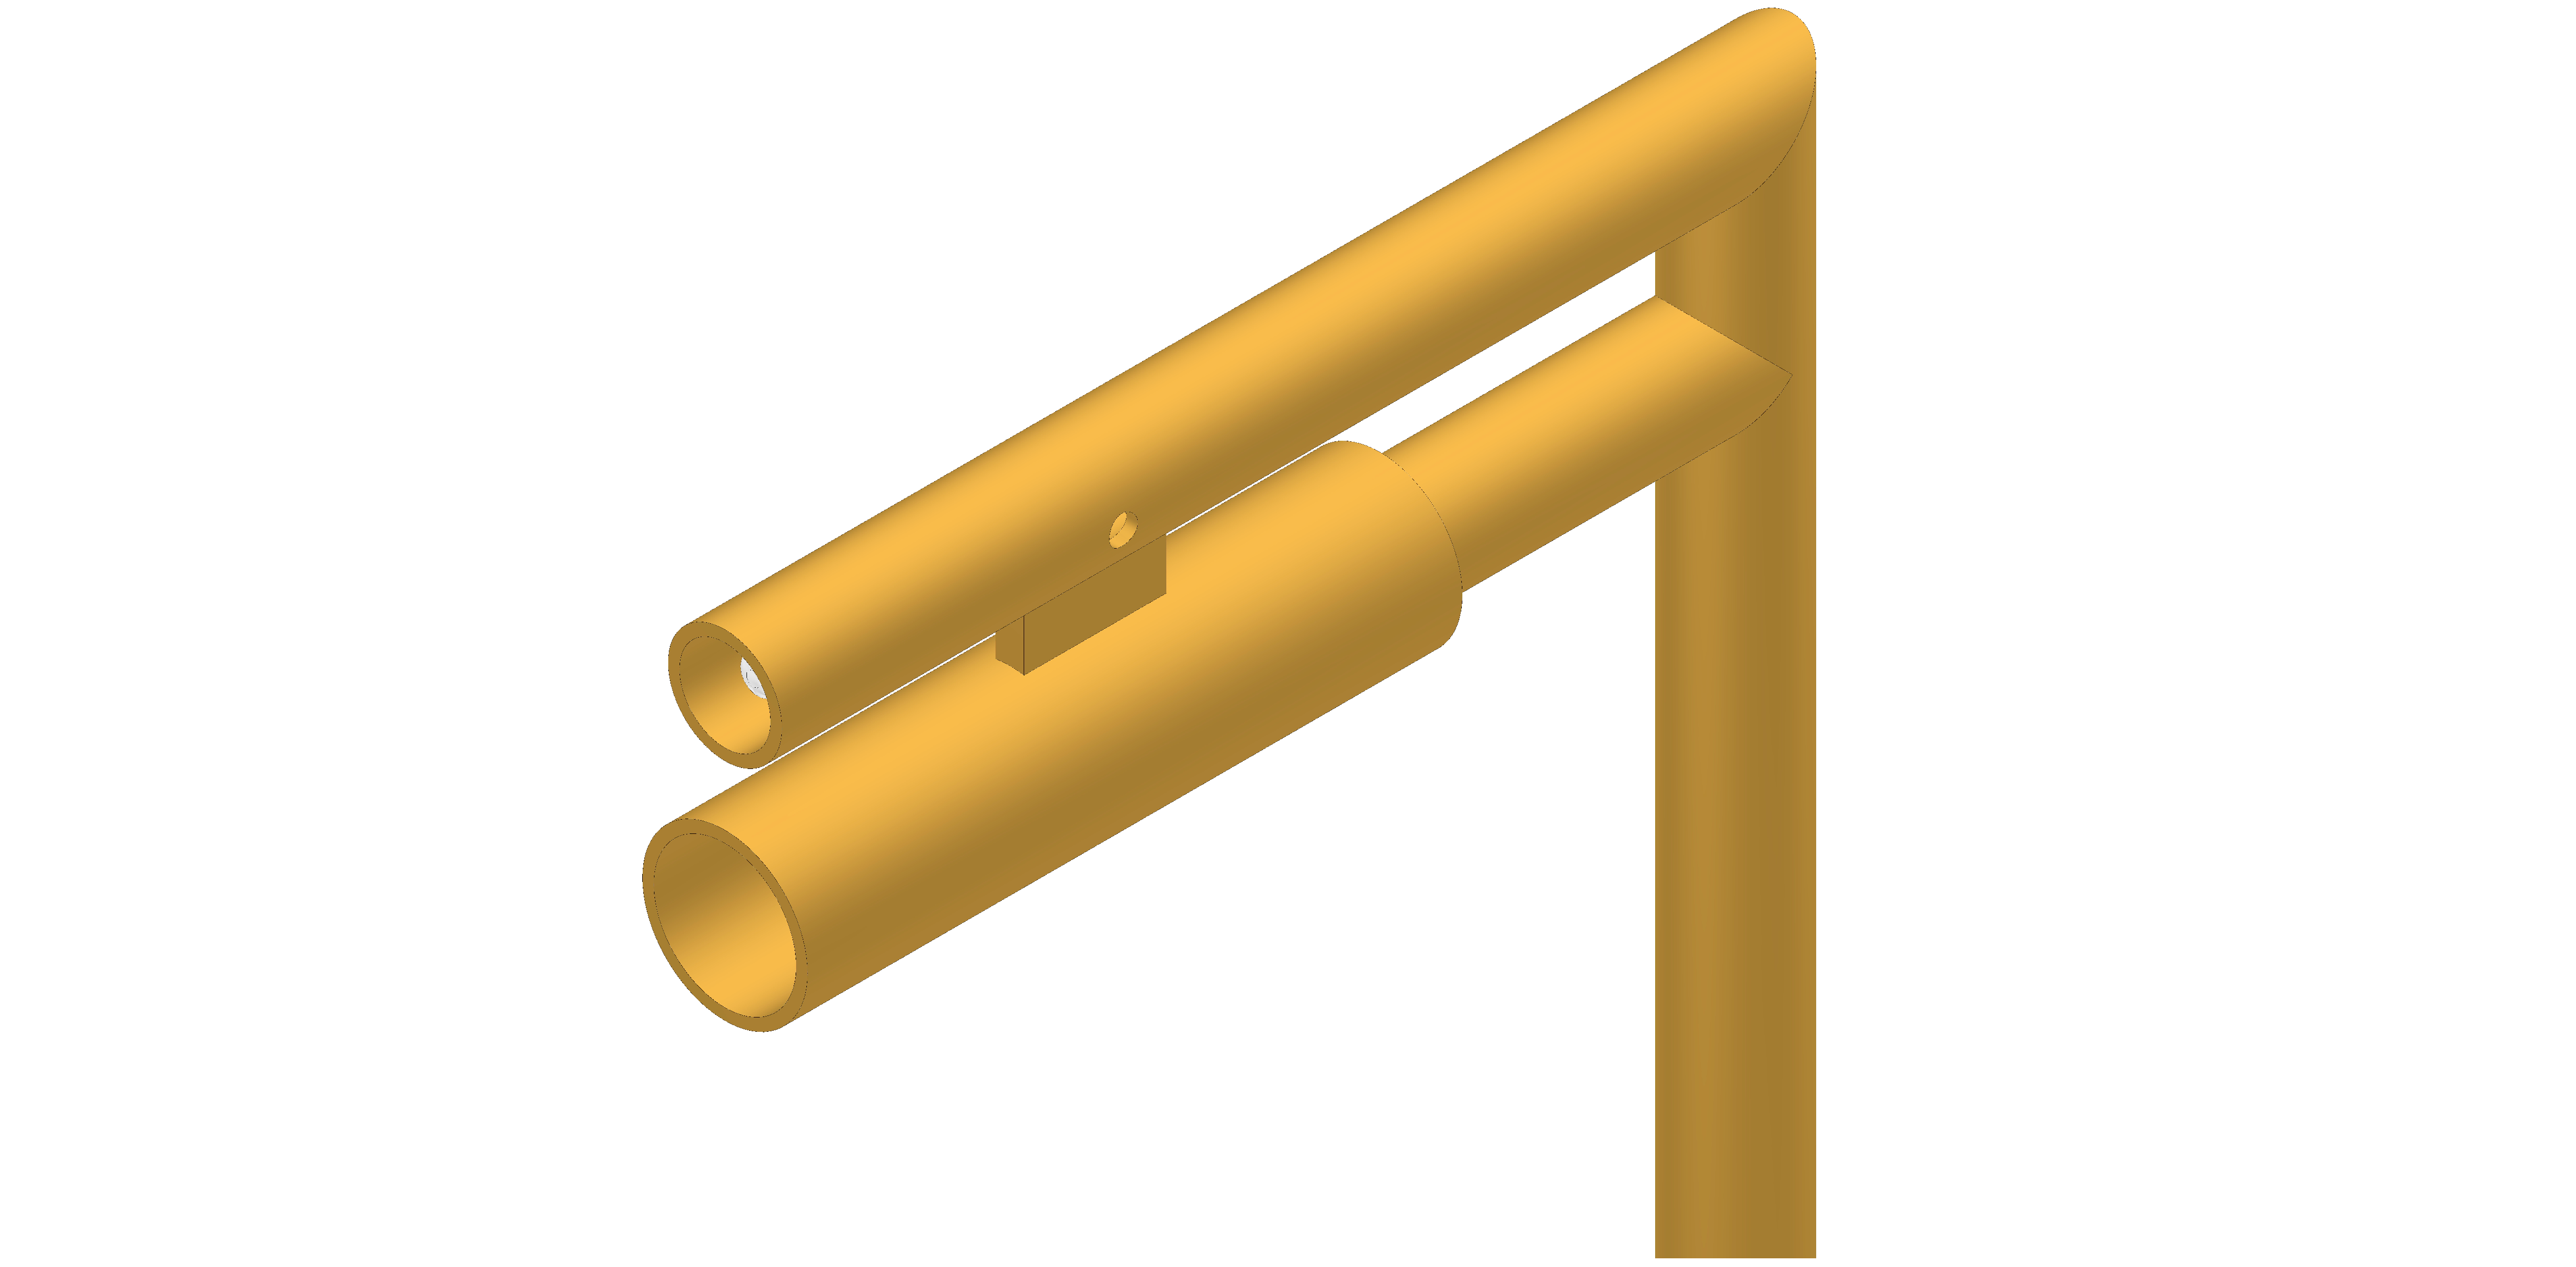
\includegraphics[width=\textwidth]{400_SIMULACE_KONSTRUKCNICH_UPRAV/Vykresy_rendery/Sonda_se_stinenim_B.png}
            \caption{Sonda se stíněním čidla B.}
            \label{fig:sonda-se-stinenim-B}
        \end{figure}

        Pro tuto geometrii byl proveden pouze jeden výpočet, a to pro rychlost $250 \Unit{\frac{m}{s}}$. Důvodem byla volba příliš úzké stínící trubice, která způsobovala výrazně vyšší ohřev čidla B oproti původní verzi (restituční faktor narostl o $7.3 \Unit{\%})$. 

        \begin{figure}[ht!]
            \centering
            \begin{subfigure}{0.45\textwidth}
                \centering
                \captionsetup{width=.9\linewidth}
                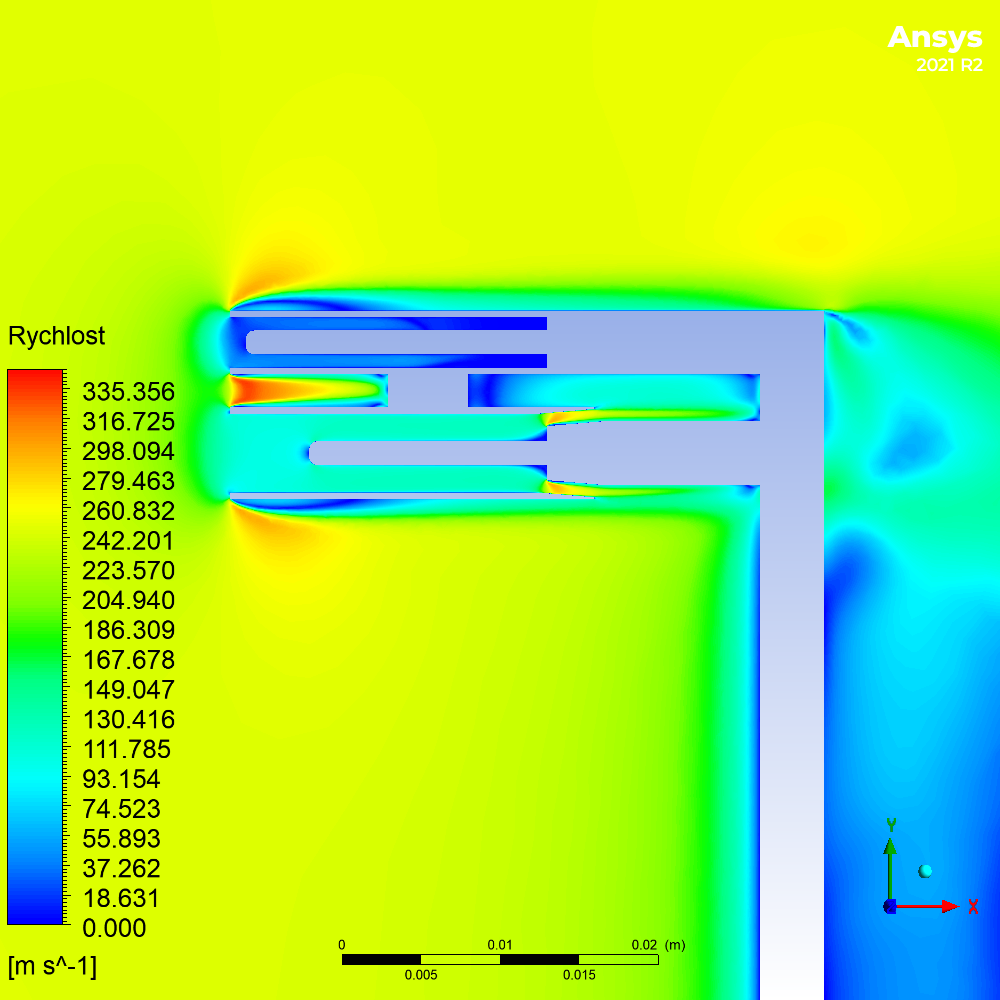
\includegraphics[width=\textwidth]{400_SIMULACE_KONSTRUKCNICH_UPRAV/Vizualizace/sonda_se_stinenim_B_vizualizace_rychlost.png}
                \caption{Rychlostní pole.}
            \end{subfigure}
            \begin{subfigure}{0.45\textwidth}
                \centering
                \captionsetup{width=.9\linewidth}
                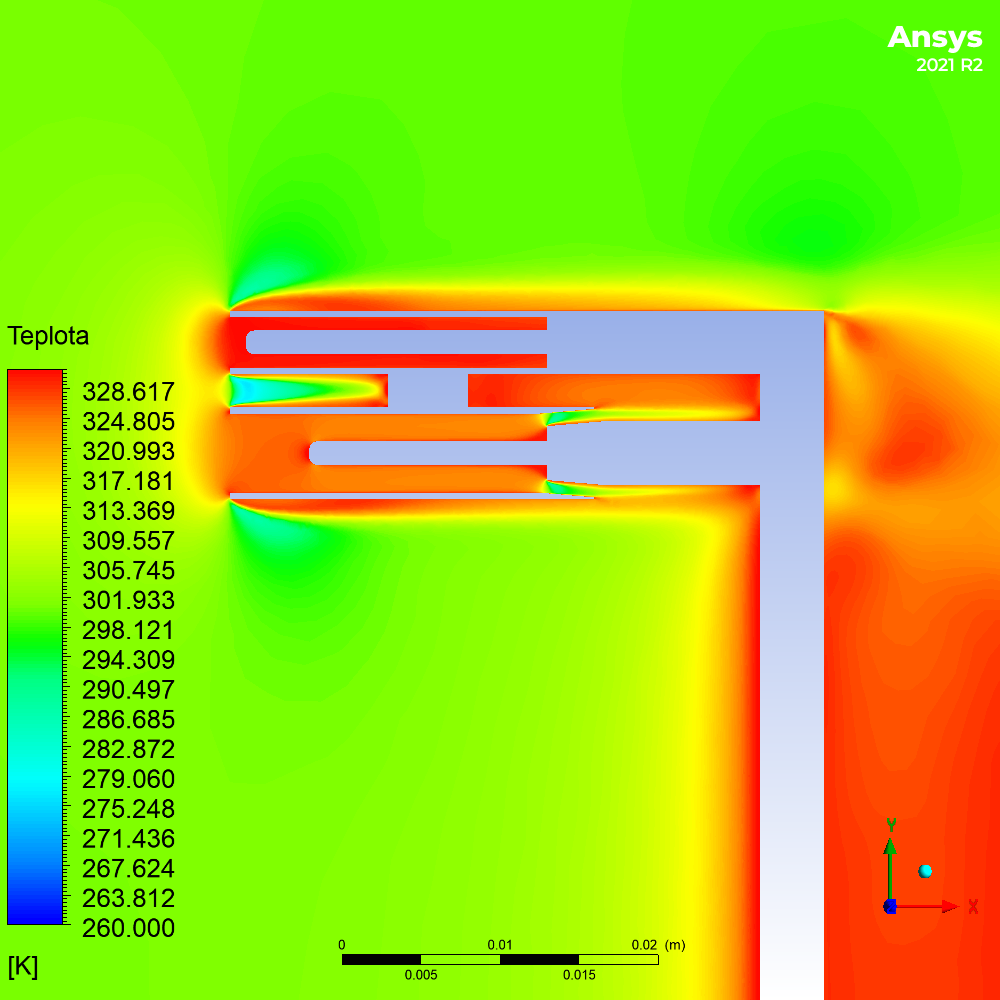
\includegraphics[width=\textwidth]{400_SIMULACE_KONSTRUKCNICH_UPRAV/Vizualizace/sonda_se_stinenim_B_vizualizace_teplota.png}
                \caption{Teplotní pole.}
            \end{subfigure}
            \caption{Vizualizace vypočtených dat pro sondu se stíněním čidla B v rovině symetrie pro rychlost proudění $250 \Unit{\frac{m}{s}}$.}
            \label{fig:sonda-se-stinenim-B-vizualizace}
        \end{figure}
    
    \newpage
    \subsection{Sonda s rozšířeným stíněním čidla B} \label{sec:sonda-s-rozsirenym-stinenim-B}
        Oproti předchozí úpravě došlo pouze ke zvětšení trubice stínící čidlo B – místo původního rozměru byla použito stínění o vnějším průměru $8 \Unit{mm}$ a tloušťce stěny $0.45 \Unit{mm}$ (geometrie podrobně popsána v Příloze \ref{fig:sonda-s-rozsirenym-stinenim-B-vykres}). Zde byl již ohřev čidla B přijatelný a bylo tak analyzováno chování sondy obdobně, jako v Kapitole \ref{sec:sonda-bez-stineni-B} – byla zkoumána závislost restitučních faktorů na rychlosti proudění v rozmezí $125 \div 325 \Unit{\frac{m}{s}}$ a na natočení v rovině symetrie a kolmo na ní, opět v rozsahu $\pm 15^o$.
        
        \begin{figure}[ht!]
            \centering
            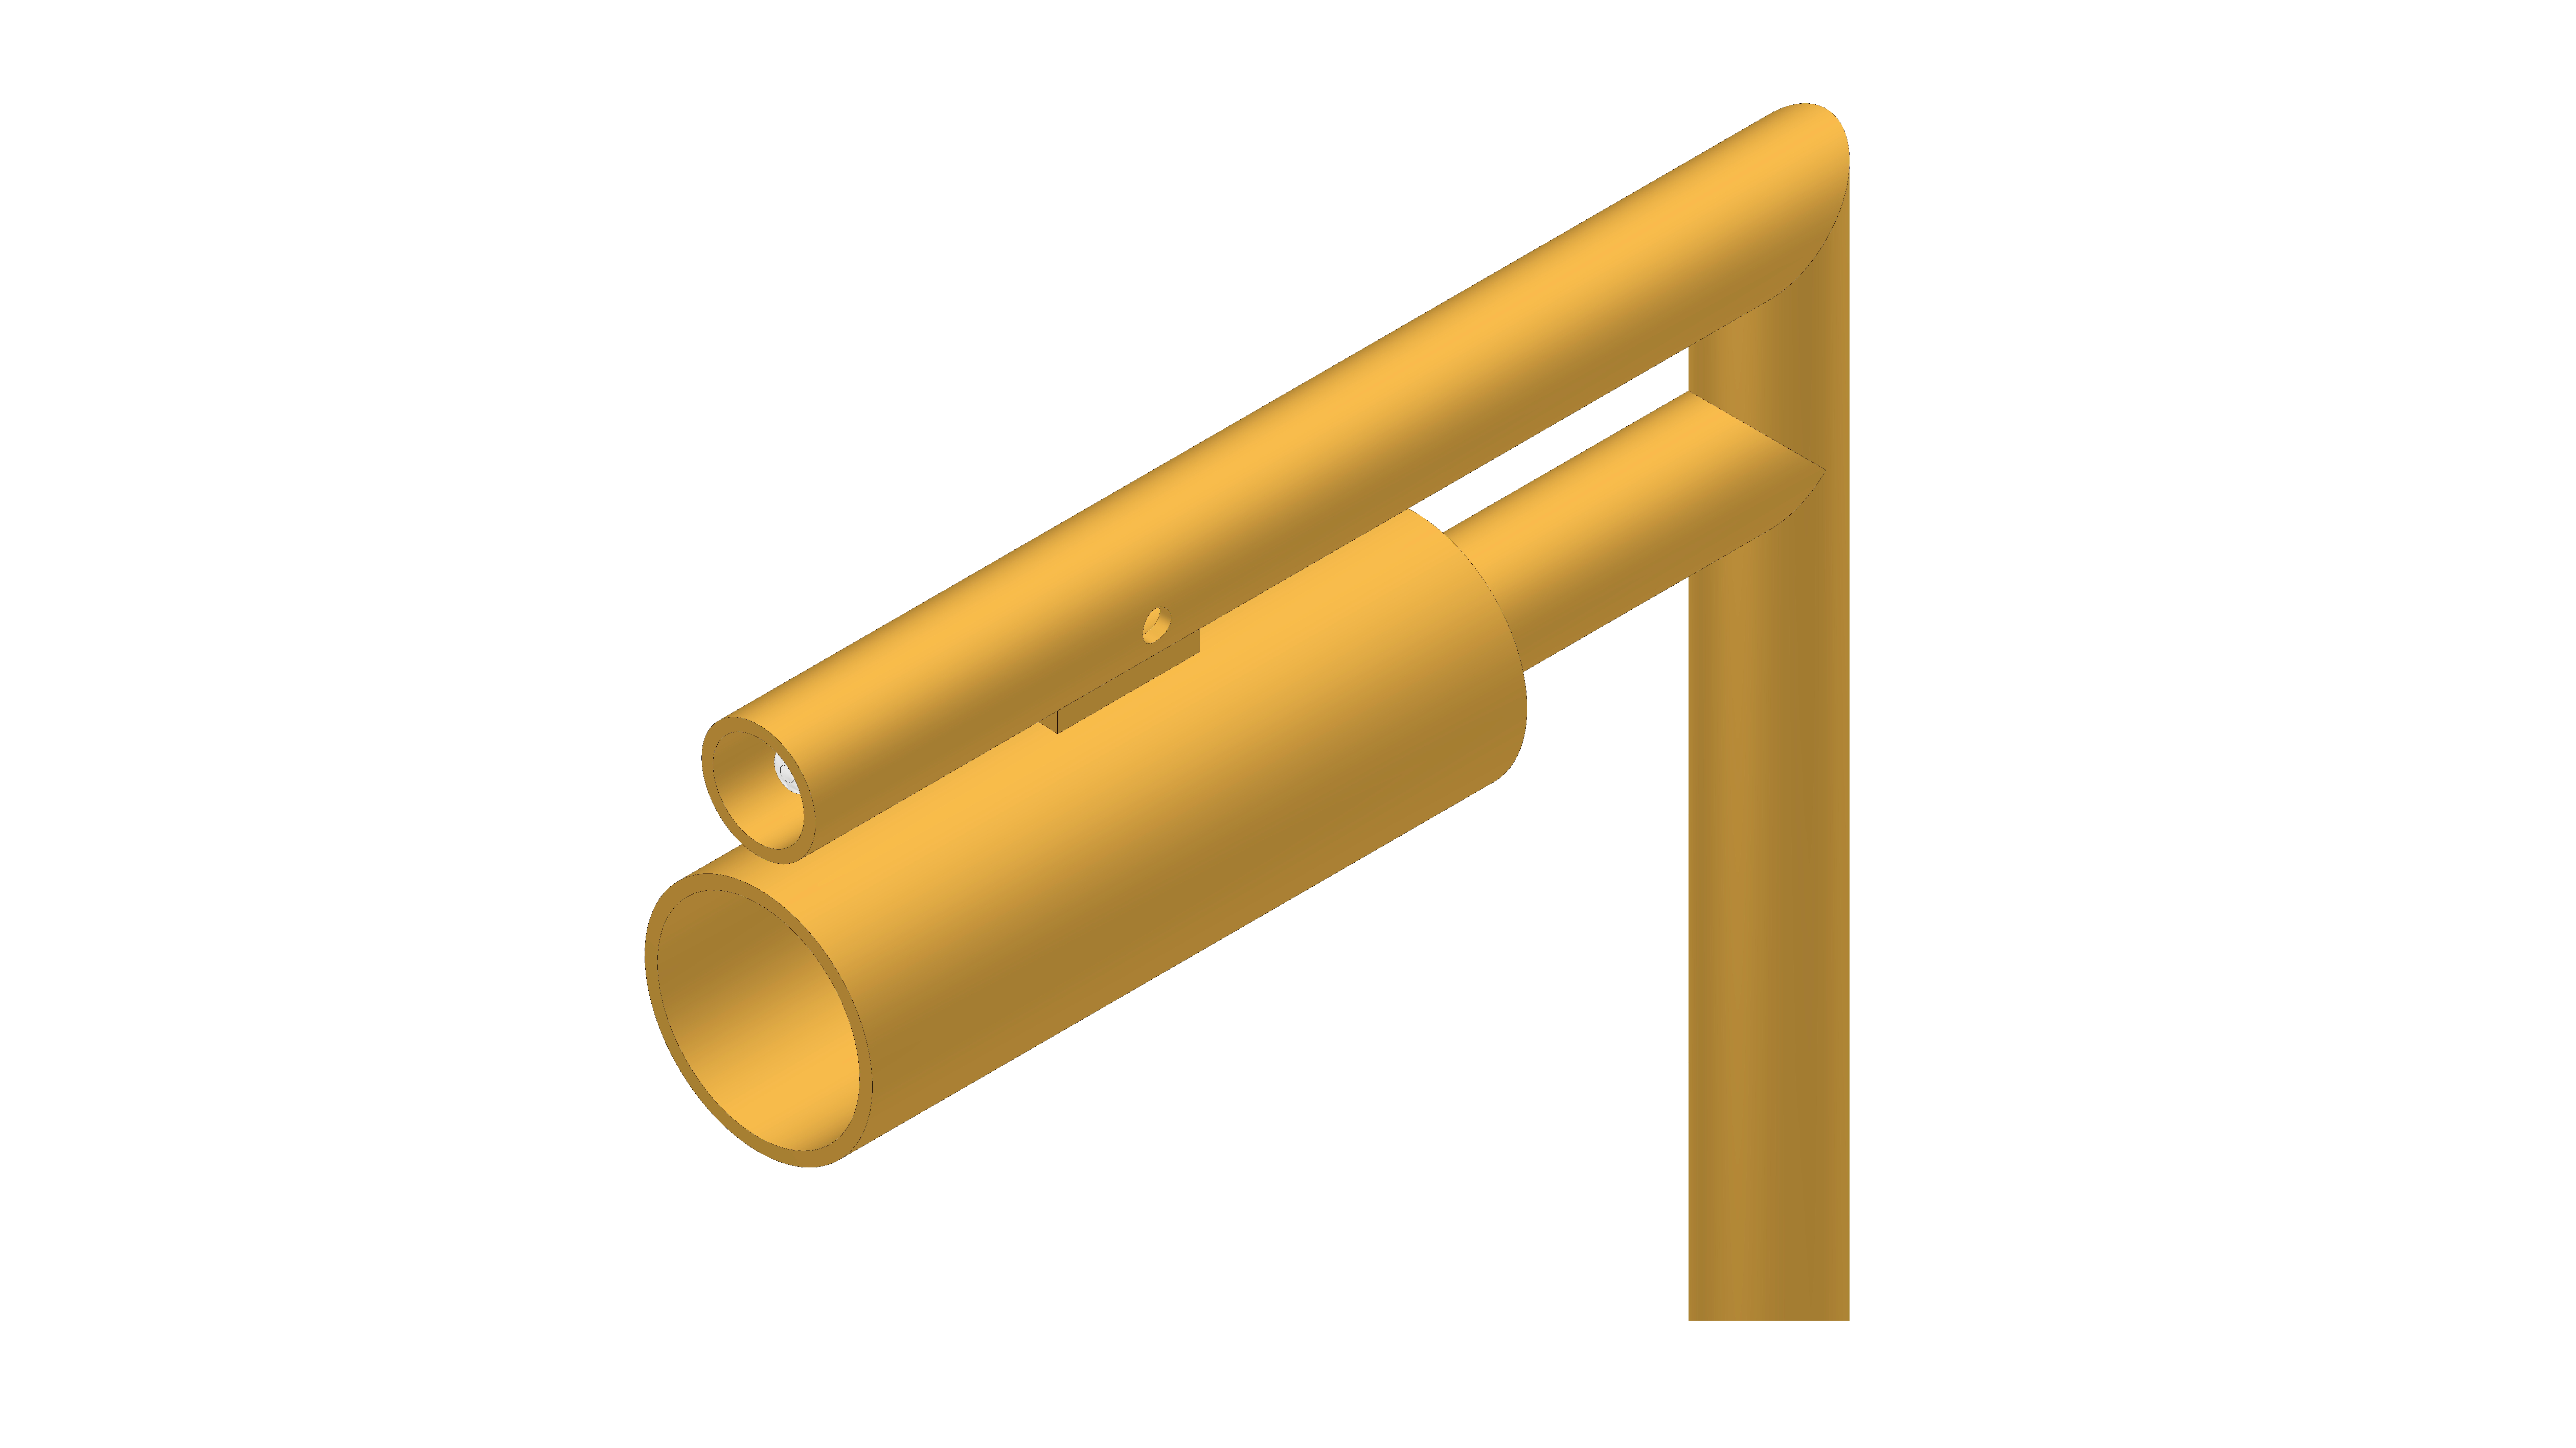
\includegraphics[width=\textwidth]{400_SIMULACE_KONSTRUKCNICH_UPRAV/Vykresy_rendery/Sonda_s_rozsirenym_stinenim_B.png}
            \caption{Sonda se stíněním čidla B.}
            \label{fig:sonda-s-rozsirenym-stinenim-B}
        \end{figure}
        
        \subsubsection{Chování při různých rychlostech proudění}
            Výsledky výpočtu shrnuje Obrázek \ref{fig:sonda-s-rosirenym-stinenim-rychlosti}. Přidáním stínící trubice došlo ke snížení vlivu stínění čidla A za cenu zvýšení restitučního faktoru čidla B, a to o přibližně $5 \Unit{\%}$.
            
            \begin{figure}[ht!]
                \centering
                \includegraphics*[width=\textwidth]{400_SIMULACE_KONSTRUKCNICH_UPRAV/Grafy/03_rychlosti.eps}
                \caption{Závislost restitučních faktorů sondy s rozšířeným stíněním čidla B na rychlosti proudění.}
                \label{fig:sonda-s-rosirenym-stinenim-rychlosti}
            \end{figure}

            \begin{figure}[ht!]
                \centering
                \begin{subfigure}{0.45\textwidth}
                    \centering
                    \captionsetup{width=.9\linewidth}
                    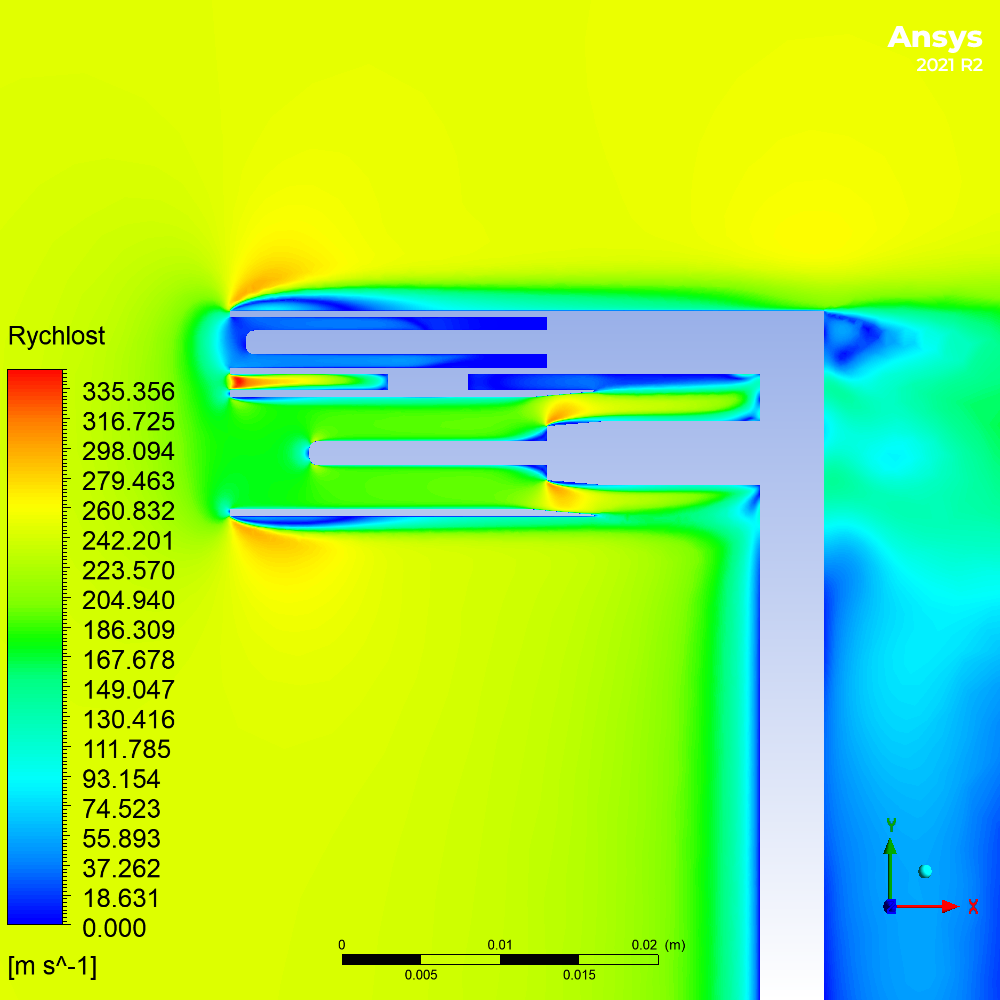
\includegraphics[width=\textwidth]{400_SIMULACE_KONSTRUKCNICH_UPRAV/Vizualizace/sonda_s_rozsirenym_stinenim_B_vizualizace_rychlost.png}
                    \caption{Rychlostní pole.}
                \end{subfigure}
                \begin{subfigure}{0.45\textwidth}
                    \centering
                    \captionsetup{width=.9\linewidth}
                    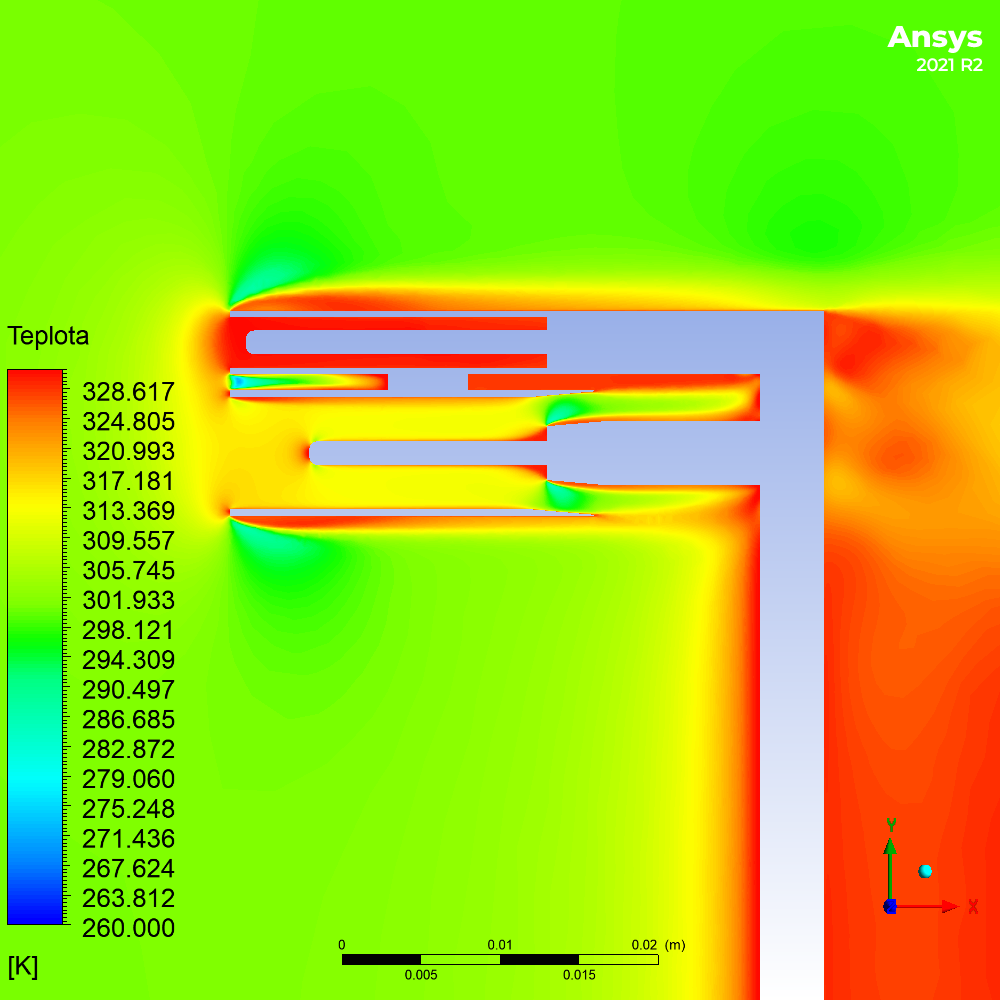
\includegraphics[width=\textwidth]{400_SIMULACE_KONSTRUKCNICH_UPRAV/Vizualizace/sonda_s_rozsirenym_stinenim_B_vizualizace_teplota.png}
                    \caption{Teplotní pole.}
                \end{subfigure}
                \caption{Vizualizace vypočtených dat pro sondu s rozšířeným stíněním čidla B v rovině symetrie pro rychlost proudění $250 \Unit{\frac{m}{s}}$.}
                \label{fig:sonda-s-rozsirenym-stinenim-B-vizualizace}
            \end{figure}
        \newpage
        \subsubsection{Směrová citlivost v rovině symetrie}
            Zde bylo zlepšení vlivem přidání stínění nejpatrnější. Restituční faktor čidla B se oproti variantě sondy bez stínění (Kapitola \ref{sec:sonda-bez-stineni-B}) vyrovnal a nedocházelo již k výraznému vlivu stínění čidla A, viz Obrázek \ref{fig:sonda-s-rosirenym-stinenim-rovina-symetrie}.
            
            \begin{figure}[ht!]
                \centering
                \includegraphics*[width=\textwidth]{400_SIMULACE_KONSTRUKCNICH_UPRAV/Grafy/03_rovina_symetrie}
                \caption{Závislost restitučních faktorů sondy s rozšířeným stíněním čidla B na natočení sondy v rovině symetrie.}
                \label{fig:sonda-s-rosirenym-stinenim-rovina-symetrie}
            \end{figure}
        \subsubsection{Směrová citlivost kolmo na rovinu symetrie}
            Výsledky výpočtů, reprezentované Obrázkem \ref{fig:sonda-s-rosirenym-stinenim-kolma-rovina}, představovaly i v tomto případě zlepšení chování restitučního faktoru čidla B, nebylo však tak výrazné, jako při natáčení sondy v rovině symetrie.
            
             \begin{figure}[ht!]
                \centering
                \includegraphics*[width=\textwidth]{400_SIMULACE_KONSTRUKCNICH_UPRAV/Grafy/03_kolma_rovina}
                \caption{Závislost restitučních faktorů sondy s rozšířeným stíněním čidla B na natočení kolmo na rovinu symetrie.}
                \label{fig:sonda-s-rosirenym-stinenim-kolma-rovina}
            \end{figure}

        \subsubsection{Zhodnocení}
            Přidáním stínění k čidlu B došlo ke snížení směrové citlivosti sondy a ke zmenšení vlivu stínění čidla A na restituční faktor čidla B. Negativním dopadem této úpravy geometrie byl vyšší ohřev čidla B, dalším krokem analýzy konstrukčních úprav tak bylo detailnější zkoumání vlivu průměru stínění čidla B na jeho restituční faktor.
    
    \newpage
    \subsection{Vliv průměru stínění čidla B}
        Čidlo B vyžadovalo stínění kvůli snížení směrové citlivosti a eliminaci vlivu trubice stínící čidlo A, dalším krokem ve zkoumání konstrukčních úprav tak bylo analyzování, jaký rozměr stínění je dostačující a jaký naopak způsobuje příliš vysoký ohřev. Podrobnější znalost této závislosti by totiž umožnila oproti předešlým kapitolám určit s\,větší jistotou rozměr stínění, který bude optimální co do míry ohřevu čidla, tak i do rozměrů stínění, které by měly být co nejmenší. 
        \begin{figure}[ht!]
            \centering
            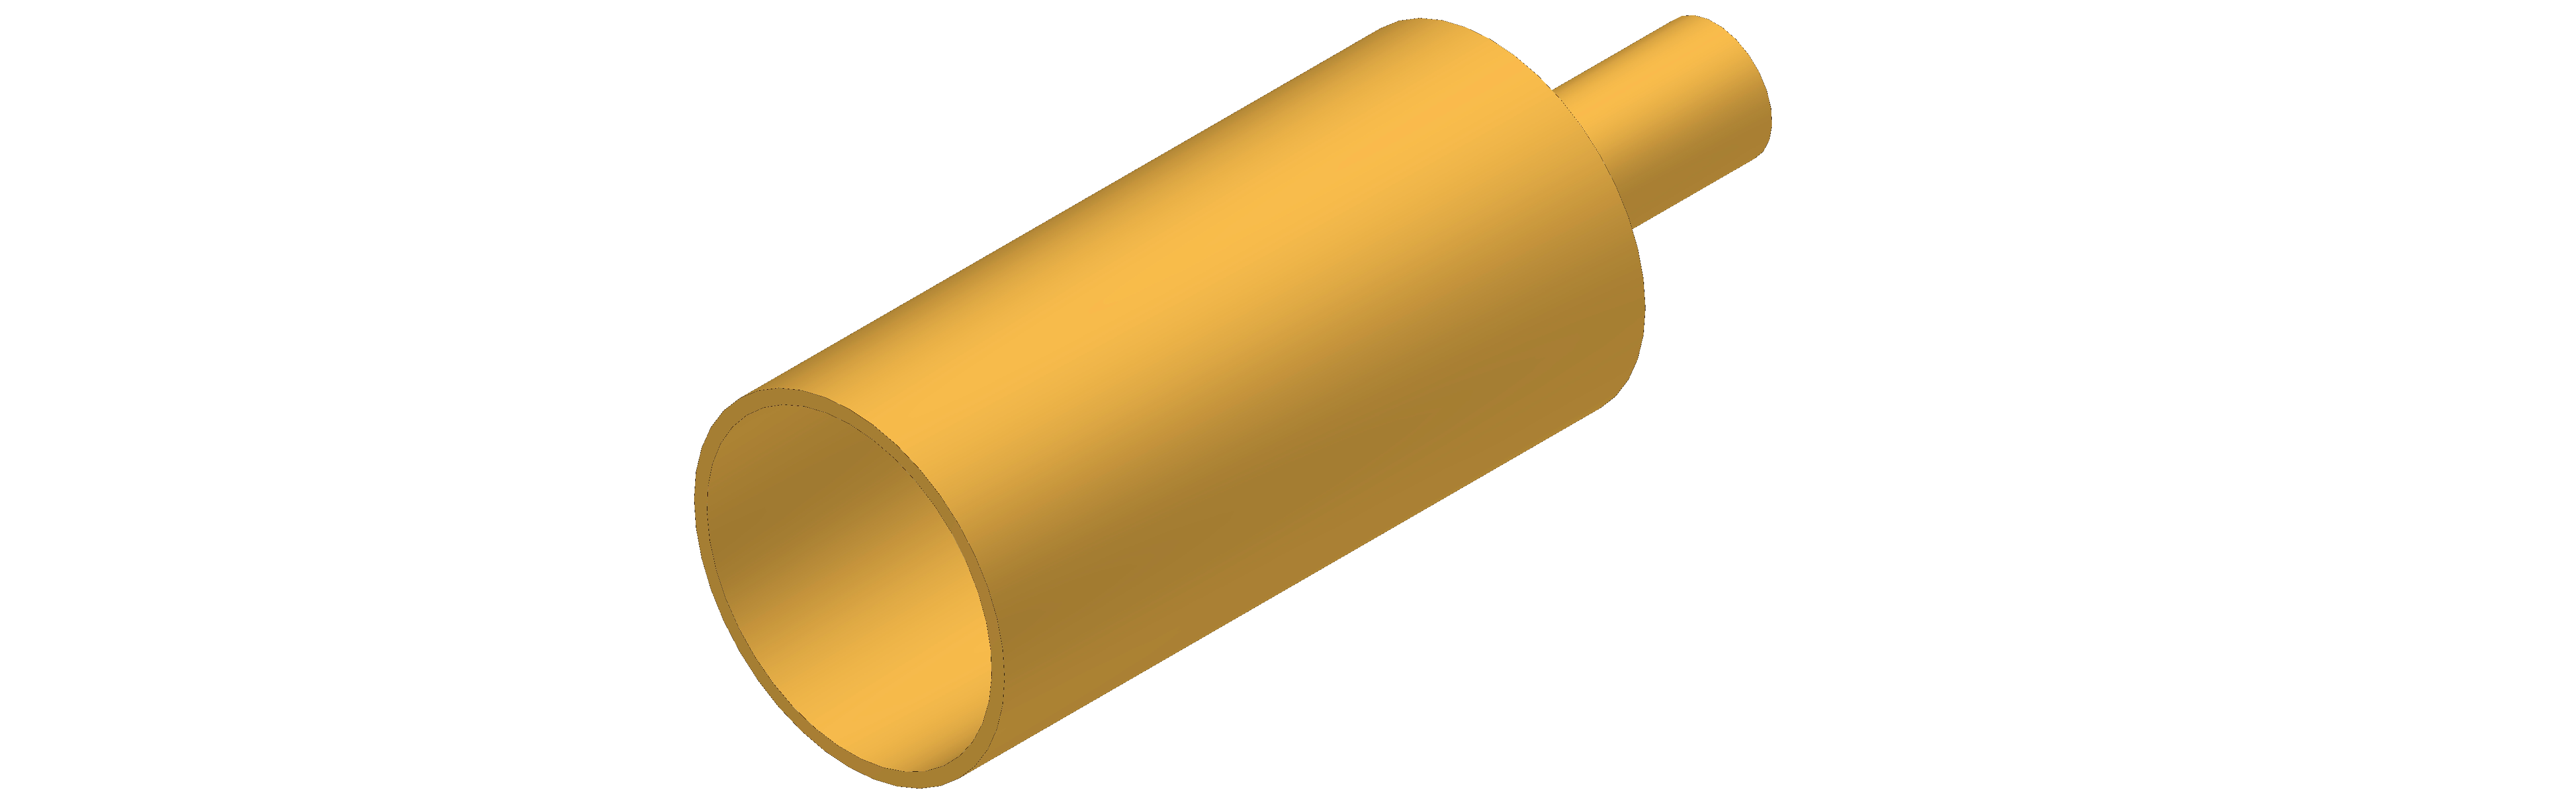
\includegraphics[width=\textwidth]{400_SIMULACE_KONSTRUKCNICH_UPRAV/Vykresy_rendery/Stineni_B.png}
            \caption{Stínění čidla B.}
            \label{fig:stineni-B}
        \end{figure}

        Zkoumáno bylo celkem 18 velikostí stínění s vnitřním průměrem v rozmezí \linebreak$3.5 \div 20\Unit{mm}$, viz výkres v Příloze \ref{fig:prumer-stineni-B-vykres}. Výpočty byly provedeny pro rychlost proudění $250 \Unit{\frac{m}{s}}$ bez natočení. Chování restitučního faktoru je patrné z Obrázku \ref{fig:prumer-stineni-B}. Od průměru $16 \Unit{mm}$ došlo k jeho ustálení, nicméně vzhledem ke snaze o zachování malých rozměrů sondy se jevily jako vhodnější průměry $7 \div 9 \Unit{mm}$, které se nachází v pásmu $2.5 \div 5 \%$ relativní odchylky od ustálené hodnoty.
        
        \begin{figure}[ht!]
            \centering
            \includegraphics*[width=\textwidth]{400_SIMULACE_KONSTRUKCNICH_UPRAV/Grafy/04_prumer_stineni_B}
            \caption{Závislost restitučního faktoru čidla B na průměru stínění.}
            \label{fig:prumer-stineni-B}
        \end{figure}
    
    \newpage
    \subsection{Vliv průměru stínění čidla A} \label{sec:stineni-A}
        Zatímco u čidla B byla snaha o dosažení co nejmenšího restitučního faktoru, pro čidlo A bylo naopak klíčové se co nejvíce příbližit měření klidové teploty ($f_A \rightarrow 1$). První analýzou zkoumající možnosti zvýšení restitučního faktoru čidla A bylo, podobně jako v předešlé kapitole, testování vlivu průměru stínící trubice. Analýza byla provedena pro celkem devět rozměrů v rozmezí $2 \div 6 \Unit{mm}$, viz Příloha \ref{fig:prumer-stineni-A-vykres}, opět pro rychlost proudění $250 \Unit{\frac{m}{s}}$ bez natočení.
        
        \begin{figure}[ht!]
            \centering
            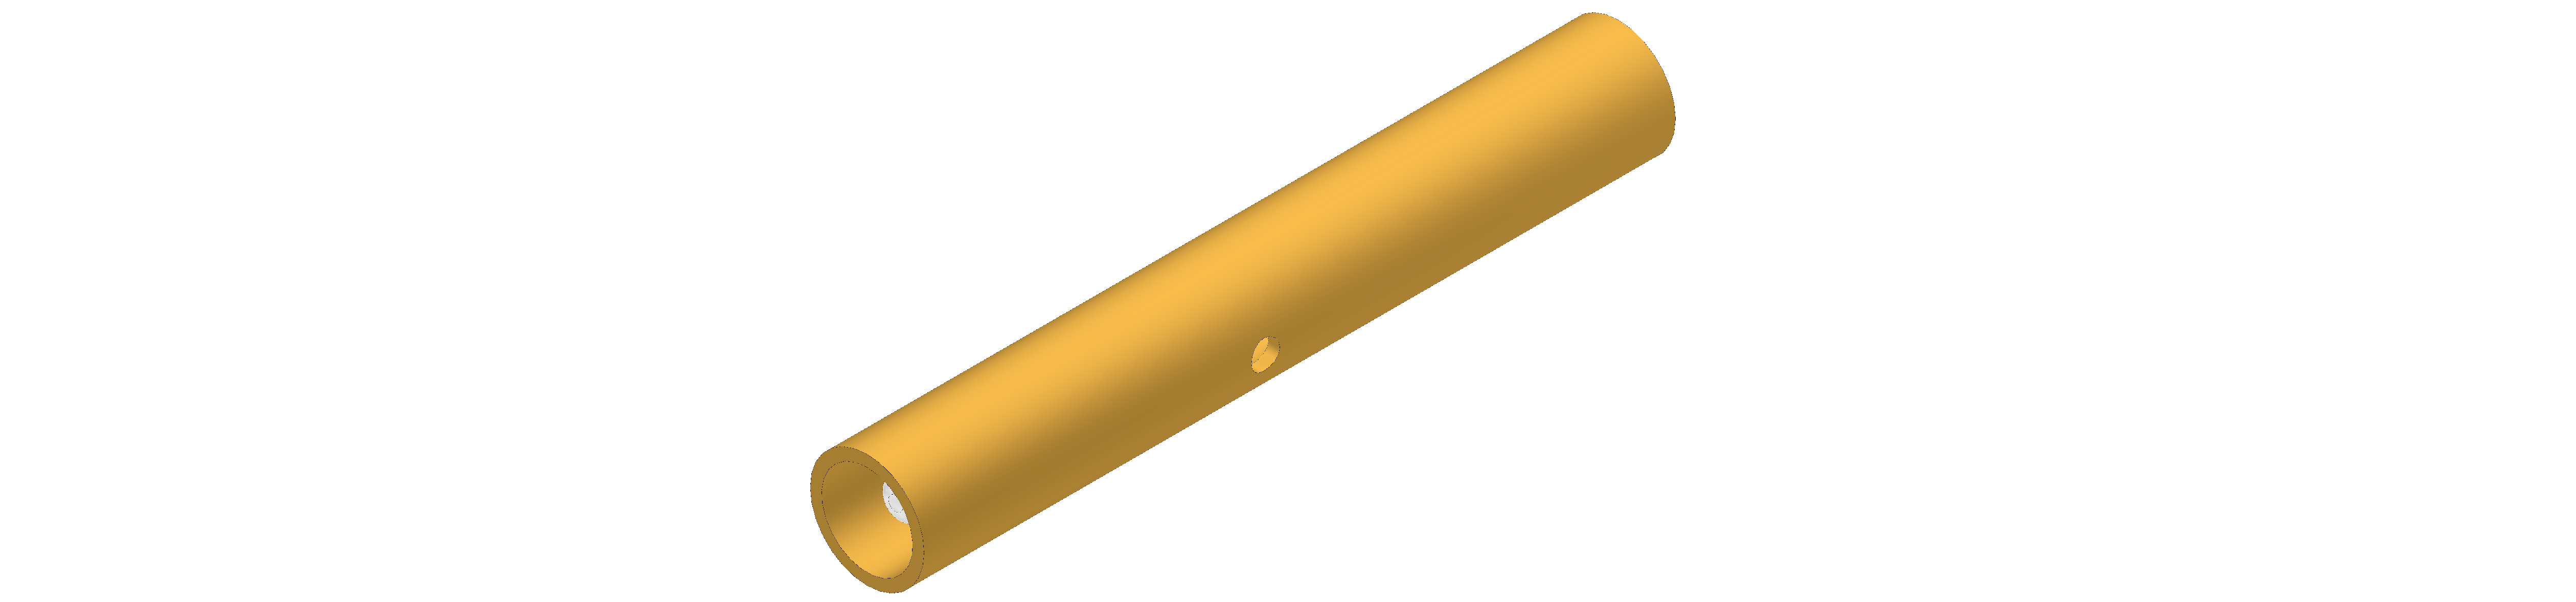
\includegraphics[width=\textwidth]{400_SIMULACE_KONSTRUKCNICH_UPRAV/Vykresy_rendery/Stineni_A.png}
            \caption{Stínění čidla A.}
            \label{fig:stineni-A}
        \end{figure}

        \newpage
        Vzhledem k tomu, že rozměr i poloha odvětrání byly zachovány, docházelo při zvětšování průměru stínění k zmenšování poměru výstupních a vstupních průřezů stínění (průměru $2 \Unit{mm}$ odpovídající poměr $0.500$ oproti průměru $6 \Unit{mm}$ s poměrem $0.0556$). Docházelo tak pravděpodobně k většímu zbrždění plynu uvitř trubice, což způsobilo nárůst měřené teploty. Vypočítané hodnoty jsou reprezentovány Obrázkem \ref{fig:prumer-stineni-A}. Zde, podobně jako u stínění čidla B, byly jako nejvhodnější (při zohlednění rozměrů a velikosti restitučního faktoru) vybrány průměry v rozmezí $3 \div 4.5 \Unit{mm}$.
        
        \begin{figure}[ht!]
            \centering
            \includegraphics*[width=\textwidth]{400_SIMULACE_KONSTRUKCNICH_UPRAV/Grafy/05_prumer_stineni_A}
            \caption{Závislost restitučního faktoru čidla A na průměru stínění.}
            \label{fig:prumer-stineni-A}
        \end{figure}
    
   \newpage
     \subsection{Vliv polohy odvětrání čidla A}
        Idea stojící za analýzou umístění odvětrání spočívala v tom, že v prostoru za odvětráním nedocházelo prakticky k žádnému proudění a nemuselo tedy docházet k optimálnímu prohřátí čidla A, které má měřicí těleso (platinový drát) umístěné podél skoro celé své délky. Zkoumán byl tak vliv polohy odvětrání, se vzdáleností od čela stínící trubice v rozmezí $2 \div 18 \Unit{mm}$, viz Výkres \ref{fig:odvetrani-A-vykres}. Průměr stínění byl shodný s původní verzí sondy, výpočty byly provedeny pro rychlost proudění $250 \Unit{\frac{m}{s}}$ bez natočení.

        Změna polohy odvětrání se ukázala v souvislosti s nárůstem restitučního faktoru čidla A jako významná, viz Obrázek \ref{fig:poloha-odvetrani-A}. Nejvyšší hodnoty bylo dosaženo umístěním $18 \Unit{mm}$ od čela stínící trubice ($2 \Unit{mm}$ před těsněním), kdy oproti původní poloze došlo k nárůstu restitučního faktoru o $1.25 \Unit{\%}$.
        
          \begin{figure}[ht!]
            \centering
            \includegraphics*[width=\textwidth]{400_SIMULACE_KONSTRUKCNICH_UPRAV/Grafy/06_poloha_odvetrani_A.eps}
            \caption{Závislost restitučního faktoru čidla A na poloze odvětrání.}
            \label{fig:poloha-odvetrani-A}
        \end{figure}
    
    \newpage
    \subsection{Vliv průměru odvětrání čidla A} \label{sec:prumer-odvetrani}
        Jak již bylo zmíněno v Kapitole \ref{sec:stineni-A}, restituční faktor čidla A byl pravděpodobně ovlivněn poměrem mezi výstupními a vstupními průřezy. Vedle změny průřezu stínící trubice lze tento poměr ovlivit i prostřednictvím různých rozměrů odvětrání, což bylo zkoumáno v této kapitole. Trubice byla použitá shodná, jako v původní verzi sondy, rozměr odvětrání byl volen v rozmezí $0 \div 1.5 \Unit{mm}$ (tedy včetně zaslepení odvětrávacích otvorů). Detailní rozměry modelu jsou uvedeny v Příloze \ref{fig:odvetrani-A-vykres}. Analýza byla provedena pro rychlost proudění $250 \Unit{\frac{m}{s}}$ bez natočení.

        Výsledky výpočtů jsou uvedeny na Obrázku \ref{fig:prumer-odvetrani-A}. Maximálního restitučního faktoru bylo dosaženo při zmenšení průměru odvětrání na $0.5 \Unit{mm}$. Při dalším zmenšování docházelo pravděpodobně k výraznému narušení proudění trubicí, což vedlo ke značnému poklesu restitučního faktoru.
        
        \begin{figure}[ht!]
            \centering
            \includegraphics*[width=\textwidth]{400_SIMULACE_KONSTRUKCNICH_UPRAV/Grafy/07_prumer_odvetrani_A.eps}
            \caption{Závislost restitučního faktoru čidla A na průměru odvětrání.}
            \label{fig:prumer-odvetrani-A}
        \end{figure}
    
    \newpage
    \subsection{Vliv přidání divergentního vstupu pro čidlo A}
        Při měření klidových teplot pomocí termočlánků se lze setkat s konstrukcemi obsahujícími vstupní difuzor, který slouží ke zbrzdění proudění. Termočlánek je poté umístěn na jeho konci \cite{Shapiro1954}. Vzhledem k charakteru geometrie čidel Pt100 nelze hovořit o bodovém měření teploty, takže jeho umístění by bylo v rámci konstrukce pro termočlánek problematické. Samotná myšlenka zpomalení proudění prostřednictvím difuzoru však představovala možnost, jak zvýšit restituční faktor čidla A. Testování této úpravy bylo provedeno pro vrcholové úhly difuzoru v rozmezí $2^o \div 12^o$, detailní popis geometrie je uveden v Příloze \ref{fig:difuzor-A-vykres}. Rychlost proudění byla shodná s předešlými simulacemi ($250 \Unit{\frac{m}{s}}$).
        
        \begin{figure}[ht!]
            \centering
            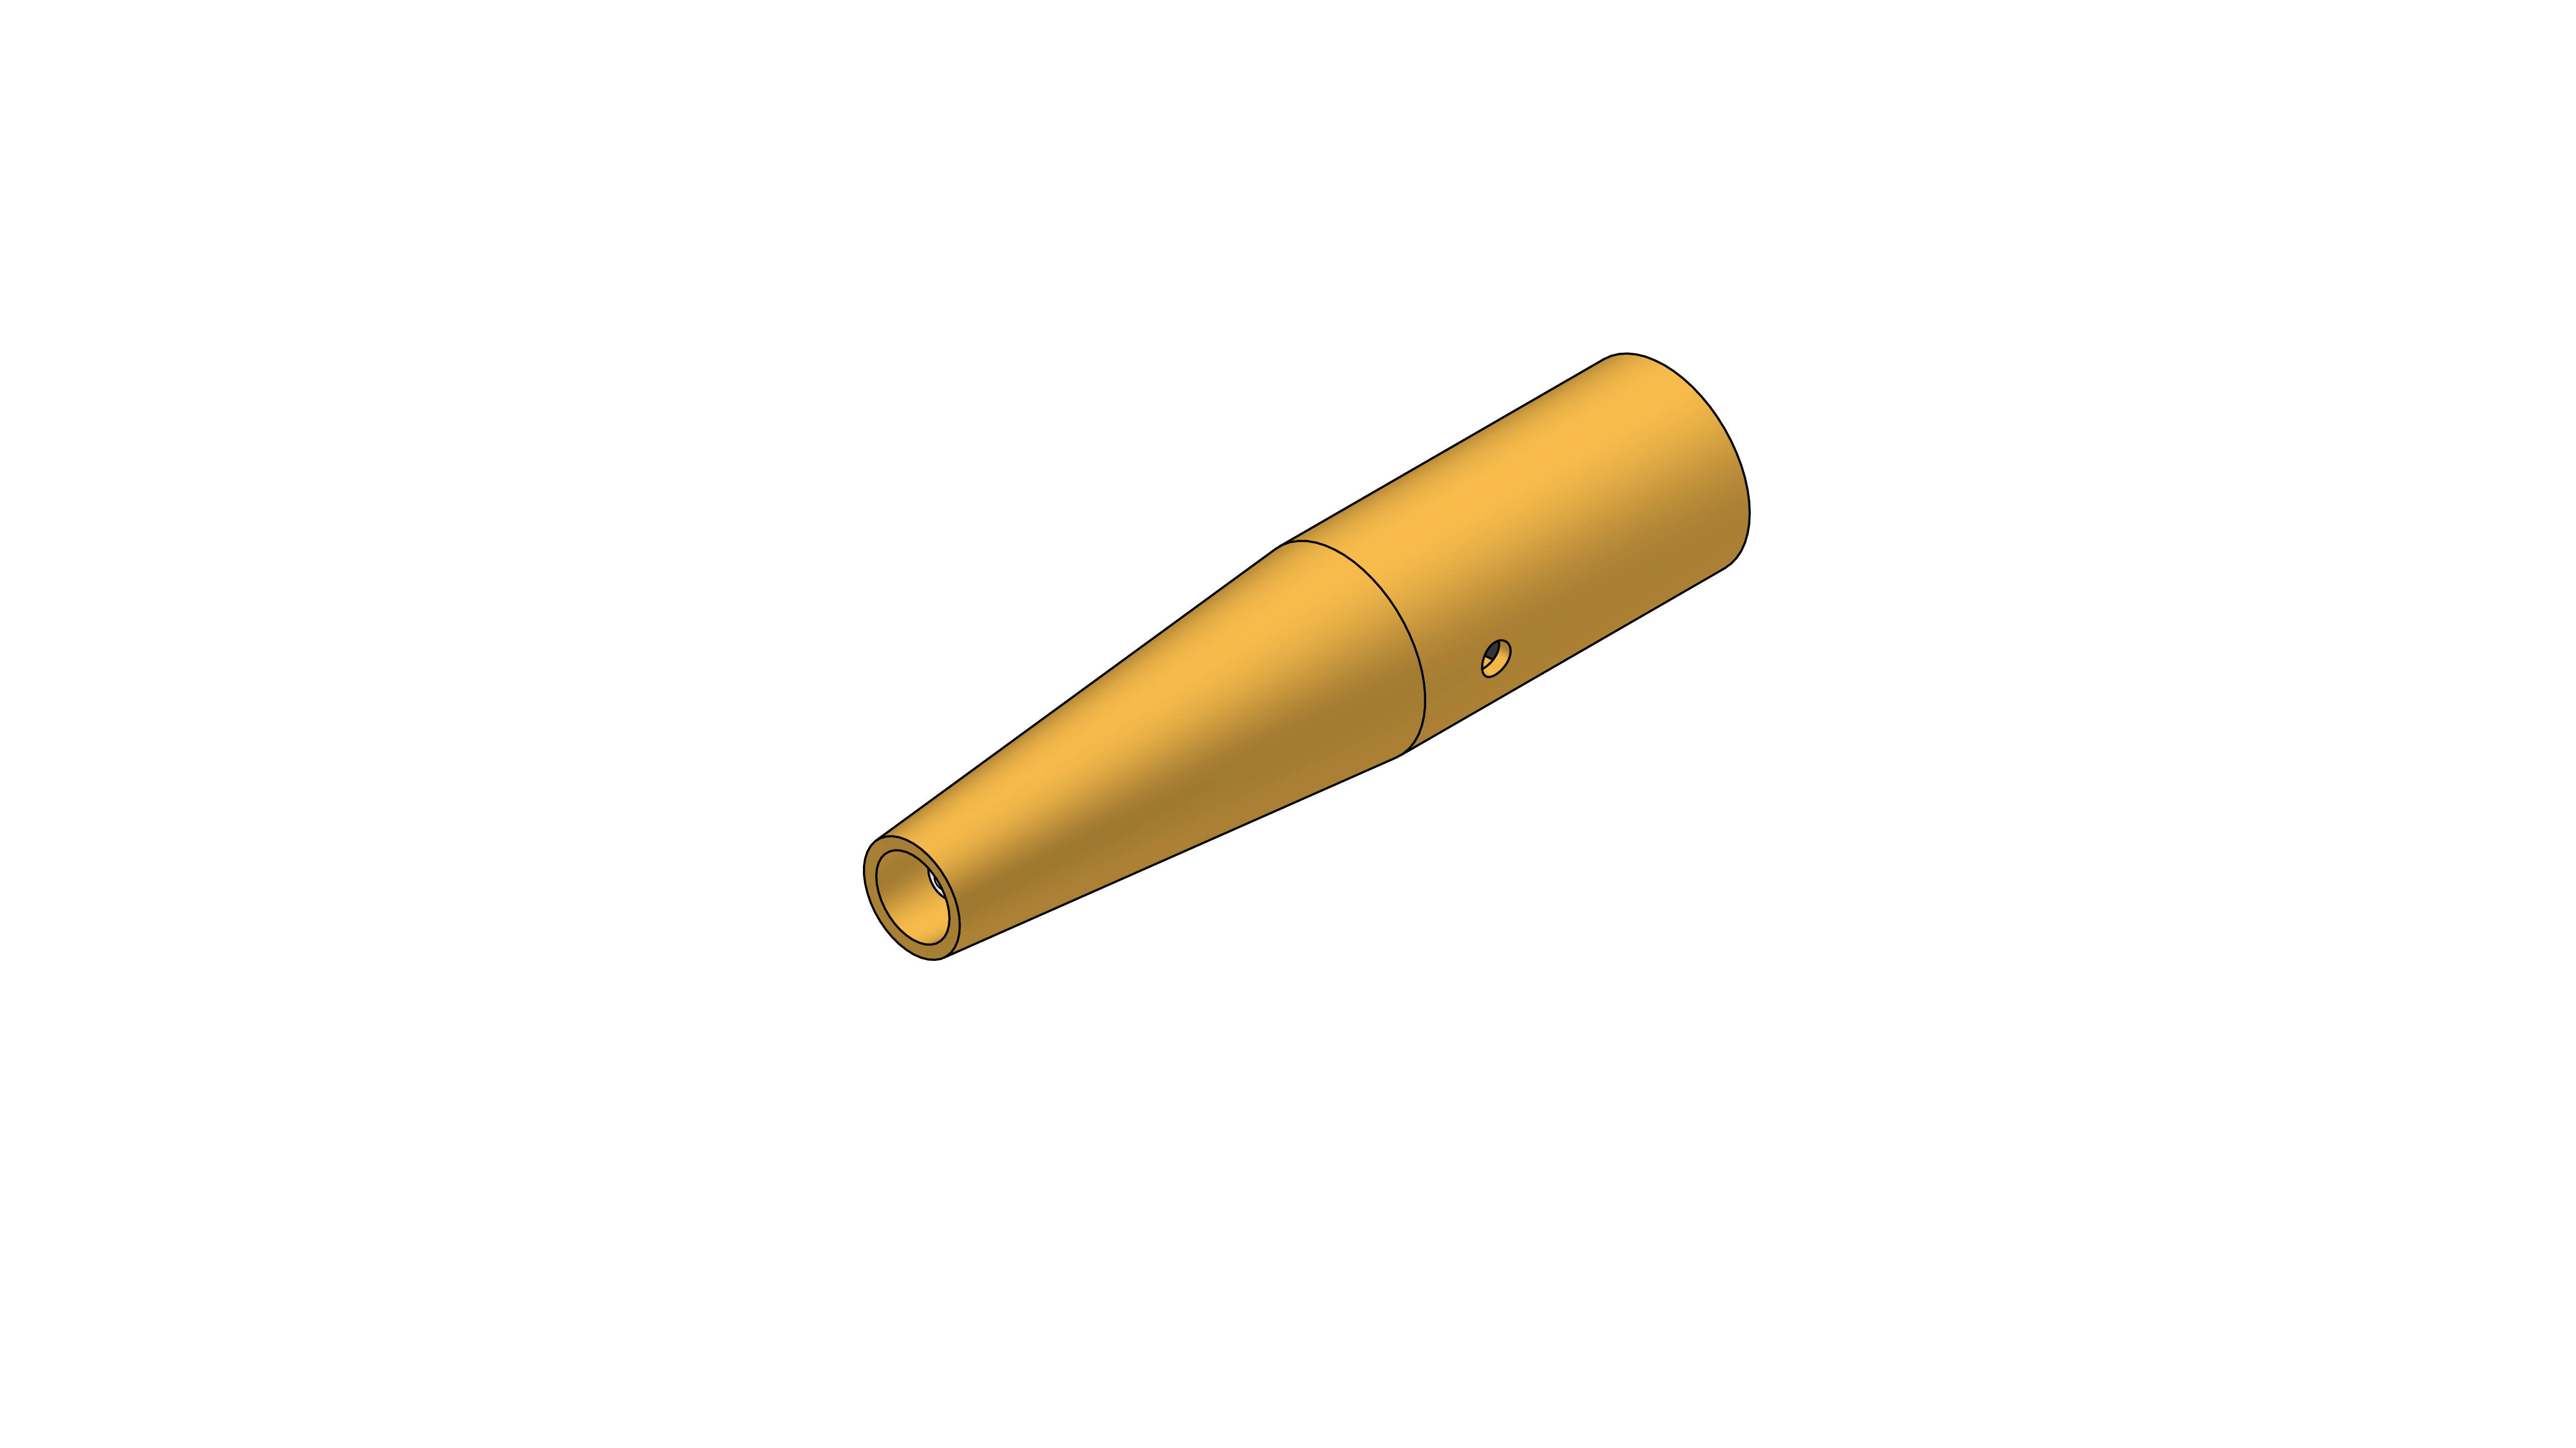
\includegraphics[width=\textwidth]{400_SIMULACE_KONSTRUKCNICH_UPRAV/Vykresy_rendery/Difuzor_A.png}
            \caption{Čidlo A s divergentním vstupem.}
            \label{fig:difuzor-A}
        \end{figure}

        Výsledky simulací (viz Obrázek \ref{fig:divergentni-cast-A}) nepotvrdily vhodnost přidání divergentní části ke stínění čidla A. S rostoucím vrcholovým úhlem docházelo k poklesu restitučního faktoru, jehož velikost (lišící se od předešlých kapitol) lze vysvětlit použitím větší trubice s\,odvětráním těsně před těsněním (oba faktory přispěly k nárůstu restitučního faktoru).
    
        \begin{figure}[ht!]
            \centering
            \includegraphics*[width=\textwidth]{400_SIMULACE_KONSTRUKCNICH_UPRAV/Grafy/08_divergentni_cast_A.eps}
            \caption{Závislost restitučního faktoru čidla A na vrcholovém úhlu divergentního vstupu.}
            \label{fig:divergentni-cast-A}
        \end{figure}
    
    \newpage
    \subsection{Vliv přidání kavity do stínění} \label{sec:kavita}
        Poslední zkoumanou konstrukční úpravou před návrhem finální geometrie sondy bylo přidání kavity do stínění čidel – cílem bylo určit, jak moc dojde vlivem částečného odizolování od okolního proudění ke změně restitučních faktorů. Kavita ve stínění byla tvořena mezerou mezi vnitřní a vnější stěnou trubice, která byla proměnlivá v rozmezí \linebreak $0 \div 1.5 \Unit{mm}$, viz Přílohy \ref{fig:kavita-A-vykres} a \ref{fig:kavita-B-vykres} pro detailní geometrii konstrukce pro čidlo A, resp. pro čidlo B. Numerické testování probíhalo pro rychlost proudění $250 \Unit{\frac{m}{s}}$ bez natočení.

        \begin{figure}[ht!]
            \centering
            \begin{subfigure}{0.45\textwidth}
                \centering
                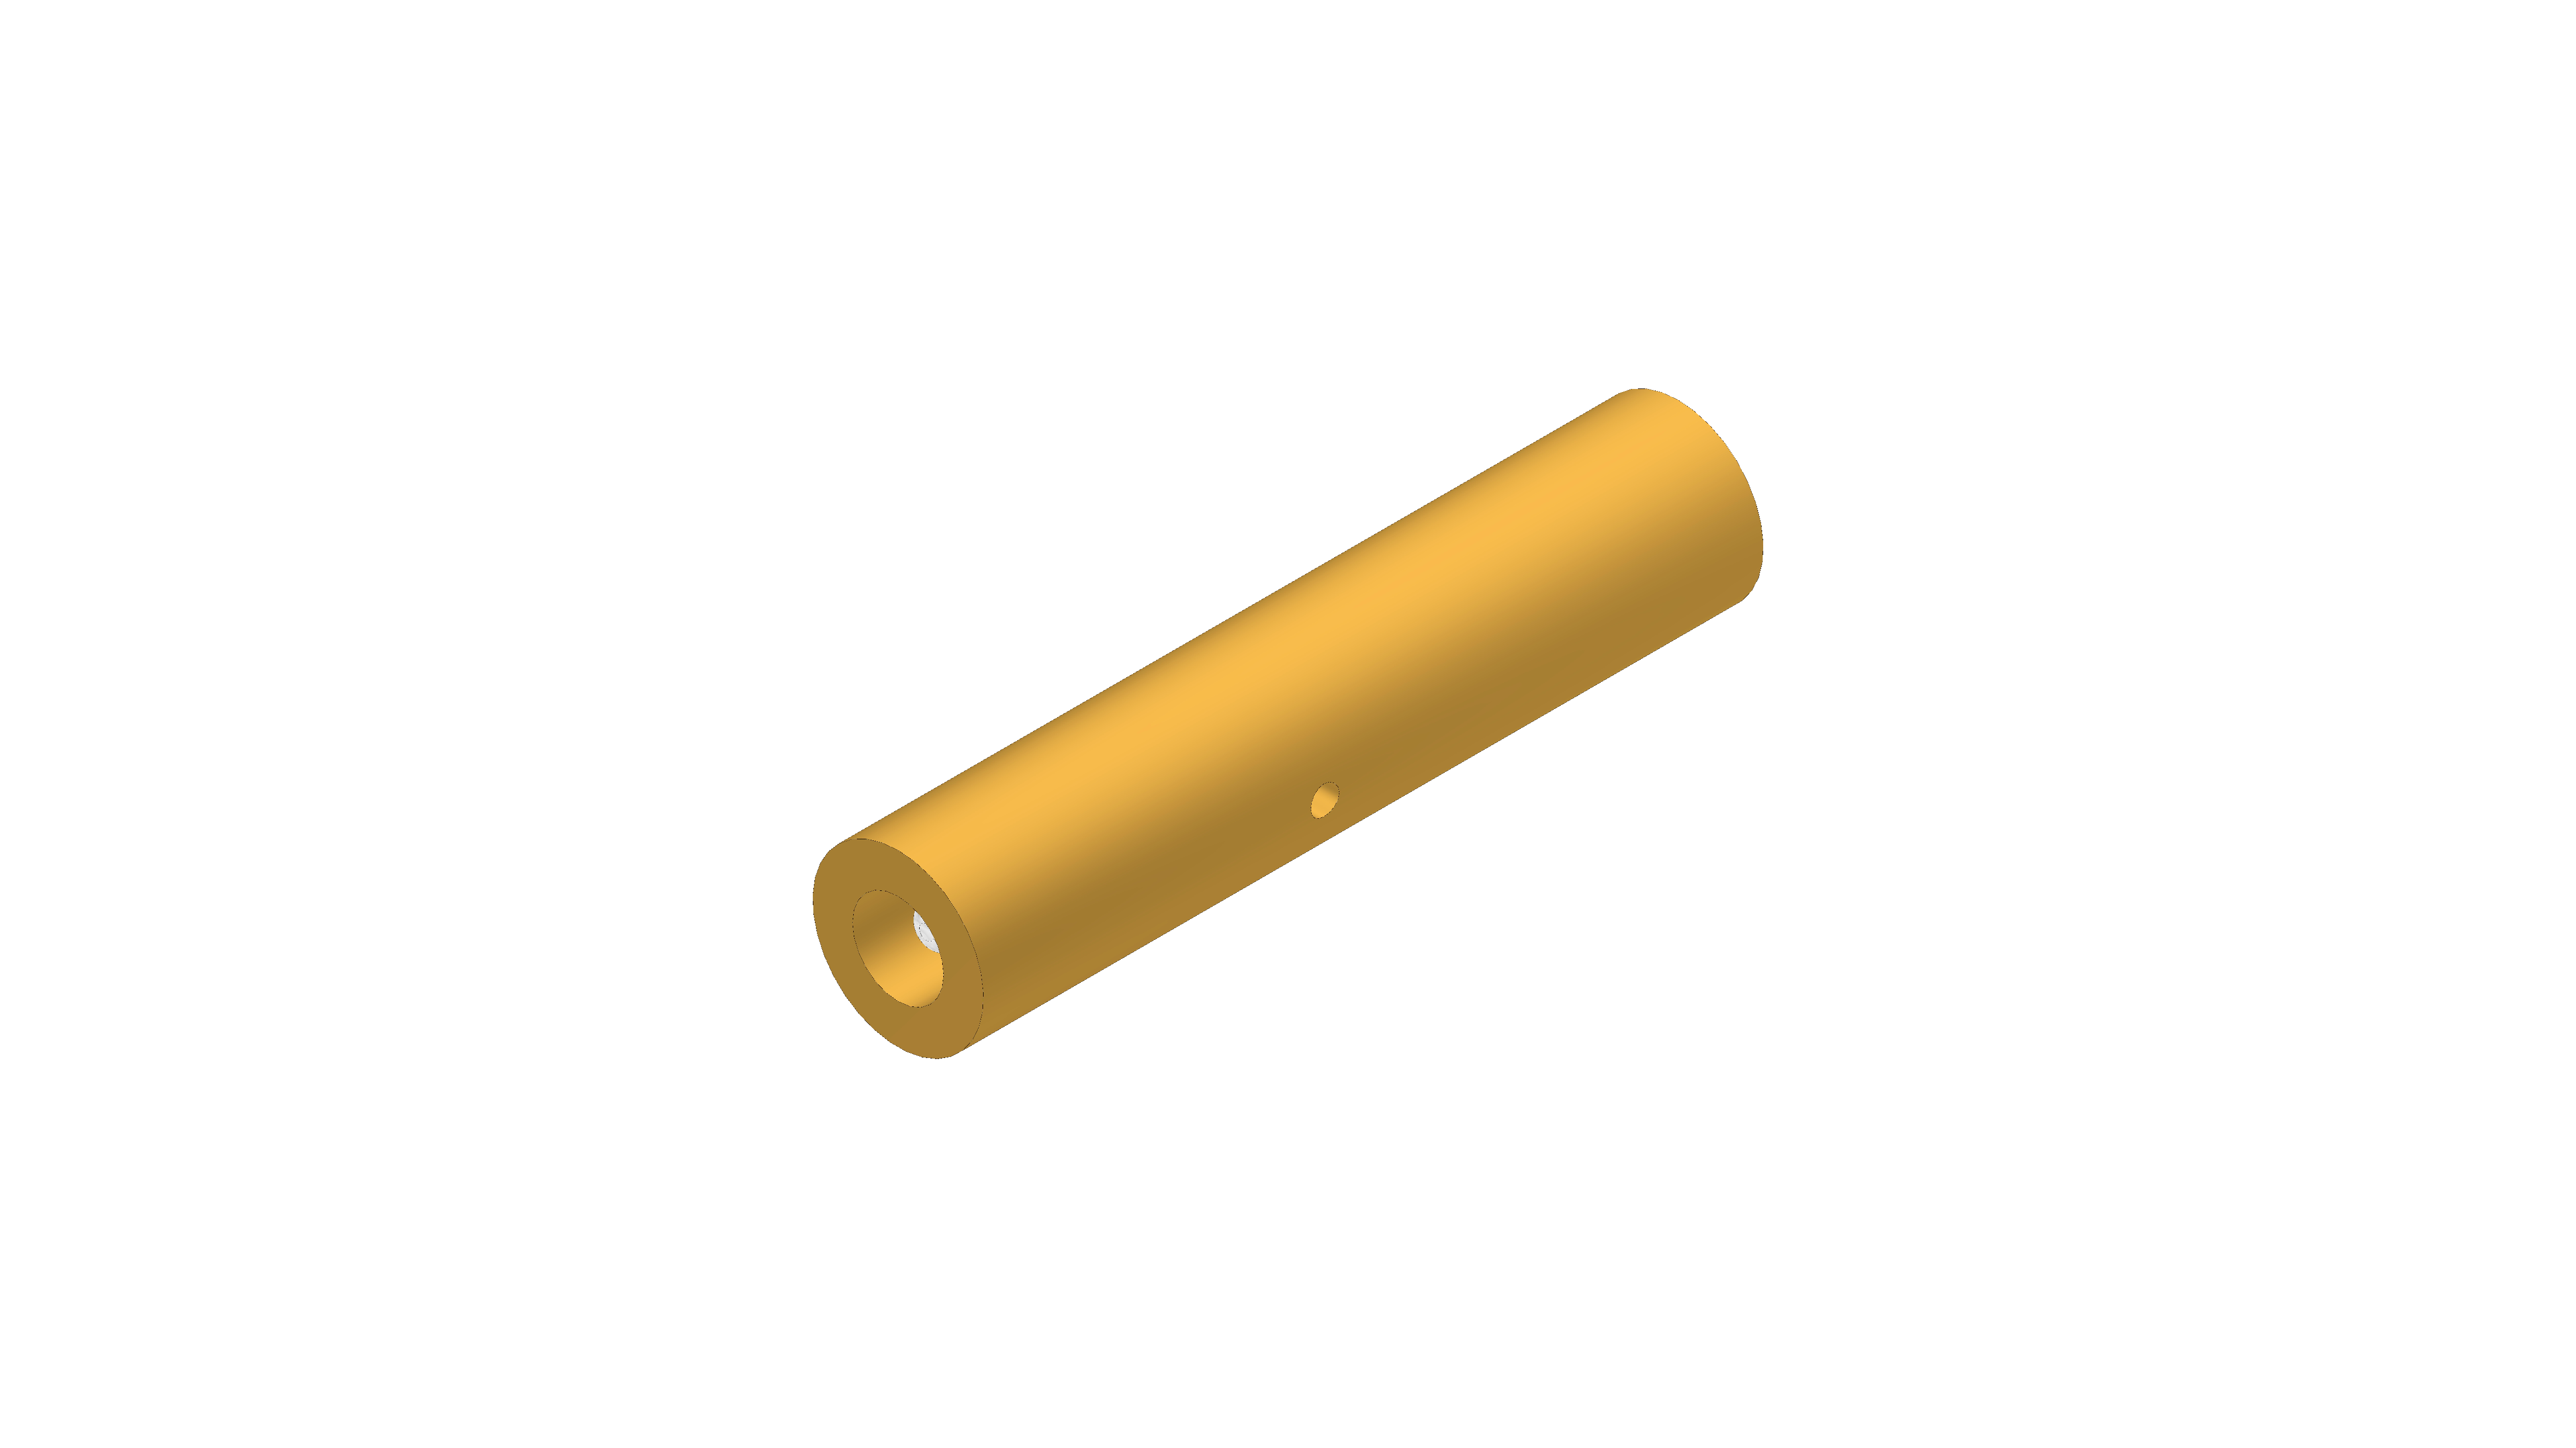
\includegraphics[width=\textwidth]{400_SIMULACE_KONSTRUKCNICH_UPRAV/Vykresy_rendery/Kavita.png}
                \caption{Čidlo A.}
                \label{fig:kavita-A}
            \end{subfigure}
            \begin{subfigure}{0.45\textwidth}
                \centering
                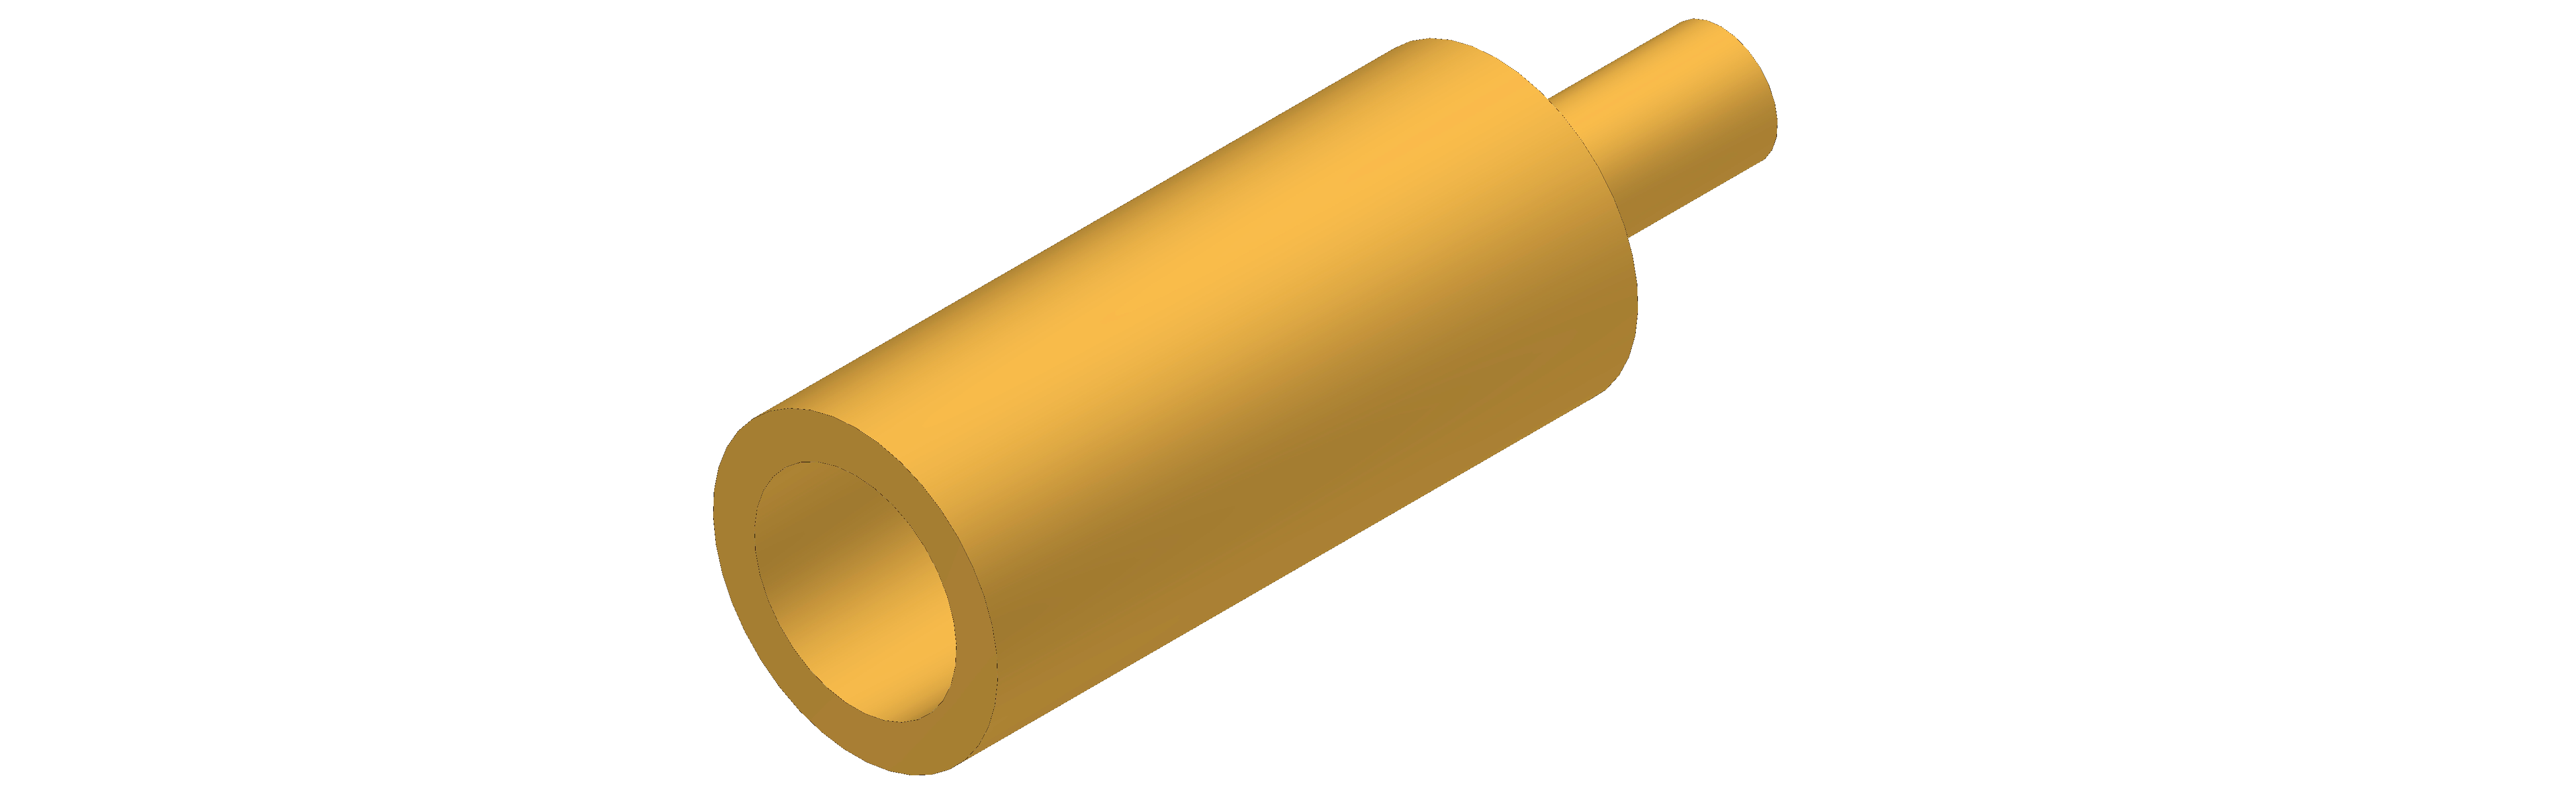
\includegraphics[width=\textwidth]{400_SIMULACE_KONSTRUKCNICH_UPRAV/Vykresy_rendery/Kavita_B.png}
                \caption{Čidlo B.}
                \label{fig:kavita-B}
            \end{subfigure}
            \caption{Modely pro testování vlivu přidání kavity do stínění.}
            \label{fig:kavita-modely}
        \end{figure}
        
        \subsubsection{Čidlo A}
            Chování restitučního faktoru, viz Obrázek \ref{fig:kavita-A-graf}, bylo přesně opačné oproti očekáváním – při odizolování vnitřního prostoru byl předpokládán pokles tepelného toku stěnou a tím pádem zachování vyšší teploty proudění. K rozporu s předpoklady mohlo dojít vlivem zvětšení geometrie, která tak více narušovala proudění v okolí čidla a jeho stínění.
            \begin{figure}[ht!]
                \centering
                \includegraphics*[width=\textwidth]{400_SIMULACE_KONSTRUKCNICH_UPRAV/Grafy/kavita.eps}
                \caption{Závislost restitučního faktoru čidla A na tloušťce kavity uvnitř stínění.}
                \label{fig:kavita-A-graf}
            \end{figure}
        
        \newpage
        
        \subsubsection{Čidlo B}
            V tomto případě výsledky odpovídají předpokladům – změna velikosti kavity ve\,stínění neměla prakticky žádný vliv na velikost restitučního faktoru čidla B, viz Obrázek \ref{fig:kavita-B-graf} (změna restitučního faktoru nepřekročila $0.4 \Unit{\%}$).
        
            \begin{figure}[ht!]
                \centering
                \includegraphics*[width=\textwidth]{400_SIMULACE_KONSTRUKCNICH_UPRAV/Grafy/kavita_B.eps}
                \caption{Závislost restitučního faktoru čidla B na tloušťce kavity uvnitř stínění.}
                \label{fig:kavita-B-graf}
            \end{figure}
    